
\documentclass[11pt]{article}

% -------------------- Page & Layout --------------------
\usepackage[margin=1in]{geometry}

% -------------------- Math Packages --------------------
\usepackage{amsmath, amssymb, amsthm}
\usepackage{mathtools}

% -------------------- Graphics & Figures --------------------
\usepackage{tikz}

\usepackage{graphicx}
\usepackage{pgfplots}
\pgfplotsset{compat=1.18}

% -------------------- Tables --------------------
\usepackage{array}
\usepackage{booktabs}

% -------------------- Misc --------------------
\usepackage{enumitem}   % better control of lists
\usepackage[colorlinks=true,linkcolor=blue,citecolor=blue,urlcolor=blue]{hyperref}

% -------------------- Theorem Styles --------------------
\newtheoremstyle{spaced}%
  {10pt}   % Space above
  {10pt}   % Space below
  {\itshape} % Body font
  {}       % Indent amount
  {\bfseries} % Theorem head font
  {.}      % Punctuation after theorem head
  {0.5em}  % Space after theorem head
  {}       % Theorem head spec

\theoremstyle{spaced}
\newtheorem{theorem}{Theorem}[section]
\newtheorem{lemma}[theorem]{Lemma}
\newtheorem{proposition}[theorem]{Proposition}
\newtheorem{corollary}[theorem]{Corollary}

\theoremstyle{definition}
\newtheorem{definition}[theorem]{Definition}

\theoremstyle{remark}
\newtheorem{remark}[theorem]{Remark}
\newtheorem{example}[theorem]{Example}

% -------------------- Title Info --------------------
\title{Diseños en tracks, patrones prohibidos y cotas de grado}
\author{Axel Fridman}

% =====================================================
\begin{document}
% =====================================================

\maketitle

\begin{abstract}
Estudiamos disposiciones ordenadas de un grafo sobre $k$ ``tracks'' (pistas)
en las que las aristas están restringidas por reglas de vecinos más cercanos.
Esta noción viene de la formulación del Investigathon en términos de patrones
coloreados prohibidos sobre tríos de vértices. Hacemos precisa la
correspondencia entre las dos formalizaciones, definimos los
\emph{diseños triplemente-legales en $k$ tracks} y después investigamos
cuántos tracks (es decir, ``colores'') hacen falta para un grafo dado.
Probamos cotas de grado, resultados de planaridad para $k\le 2$ y ejemplos
estructurales como ciclos y grafos obtenidos a partir de un camino agregando
una arista extra. En el camino resaltamos exactamente cuándo es posible
$k\le 2$ (``menos de tres colores'').
\end{abstract}

% -----------------------------------------------------
\section{Apéndice: Oráculo de Grover para Coloreo/QUBO}
% -----------------------------------------------------
\label{sec:grover-coloreo}

En el contexto de este trabajo, la búsqueda eficiente de coloraciones válidas puede abordarse mediante algoritmos cuánticos, en particular Grover, adaptando la lógica de oráculo a la estructura de tracks y coloraciones discutida en las secciones anteriores.


\tableofcontents

% =====================================================
\section{Configuración básica: tracks, orden y vecinos legales}
% =====================================================
\label{sec:basic-setup}
A lo largo de todo el trabajo, $G=(V,E)$ es un grafo simple finito no dirigido.

\subsection{Diseños ordenados en $k$ tracks}

Arrancamos con la estructura puramente combinatoria de los tracks y un orden
global.

\begin{definition}[Diseño ordenado en $k$ tracks]
Sea $k\in\mathbb{N}$. Un \emph{diseño ordenado en $k$ tracks} de un grafo
$G=(V,E)$ es un par
\[
  (\tau,p)
\]
compuesto por
\begin{itemize}[leftmargin=2em]
  \item una \emph{asignación de track}
  \[
    \tau : V \to \{1,\dots,k\},
  \]
  \item y una biyección de \emph{posiciones}
  \[
    p : V \to \{1,\dots,|V|\}.
  \]
\end{itemize}
Escribimos $x<y$ si y sólo si $p(x)<p(y)$ y pensamos a todos los vértices
puestos de izquierda a derecha de acuerdo a $p$.
\end{definition} 
Un ejemplo se muestra en la Figura~\ref{fig:tracks-basic}.
\begin{figure}[ht]
  \centering
  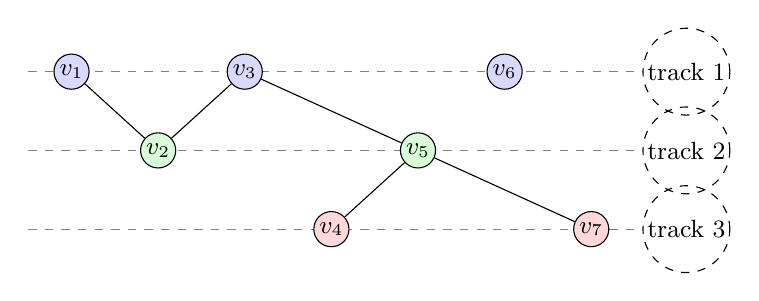
\begin{tikzpicture}[x=1.1cm,y=1cm,
    every node/.style={circle,draw,inner sep=1pt,font=\small}]
    % Track lines
    \foreach \t/\y in {1/2.0,2/1.0,3/0.0} {
      \draw[dashed,gray] (0.5,\y) -- (7.5,\y)
        node[right=1mm,black] {$\text{track }\t$};
    }

    % Vertices in global order (p(v_i) = i)
    \node[fill=blue!15]  (v1) at (1,2.0) {$v_1$};
    \node[fill=green!15] (v2) at (2,1.0) {$v_2$};
    \node[fill=blue!15]  (v3) at (3,2.0) {$v_3$};
    \node[fill=red!15]   (v4) at (4,0.0) {$v_4$};
    \node[fill=green!15] (v5) at (5,1.0) {$v_5$};
    \node[fill=blue!15]  (v6) at (6,2.0) {$v_6$};
    \node[fill=red!15]   (v7) at (7,0.0) {$v_7$};

    % Sample edges
    \draw (v1) -- (v2);
    \draw (v2) -- (v3);
    \draw (v3) -- (v5);
    \draw (v4) -- (v5);
    \draw (v5) -- (v7);
  \end{tikzpicture}
  \caption{Ejemplo de un diseño ordenado en $3$ tracks: el orden global es de izquierda a derecha, los colores indican la asignación de track $\tau$.}
  \label{fig:tracks-basic}
\end{figure}

Para cada track $t\in\{1,\dots,k\}$ definimos el conjunto de vértices
\[
  V_t := \{v\in V : \tau(v) = t\},
\]
ordenado por el $p(\cdot)$ creciente a lo largo de ese track.

\begin{definition}[Predecesor y sucesor en un track]
Dado un diseño en $k$ tracks $(\tau,p)$, un vértice $v\in V$ y un track $t$,
definimos:
\begin{align*}
  \operatorname{pred}_t(v) 
  &:= \text{el vértice en $V_t$ con mayor $p(\cdot)$ estrictamente menor que $p(v)$ (si existe)},\\
  \operatorname{succ}_t(v) 
  &:= \text{el vértice en $V_t$ con menor $p(\cdot)$ estrictamente mayor que $p(v)$ (si existe)}.
\end{align*}
Si un vértice así no existe, el predecesor/sucesor se dice
``inexistente''. Intuitivamente, son los vecinos más cercanos de $v$ sobre
el track $t$ a la izquierda/derecha en el orden global.
\end{definition} 
Ver la Figura~\ref{fig:predsucc} para una vista pictórica sobre un solo track.
\par\vspace{1em}


\begin{figure}[ht]
  \centering
  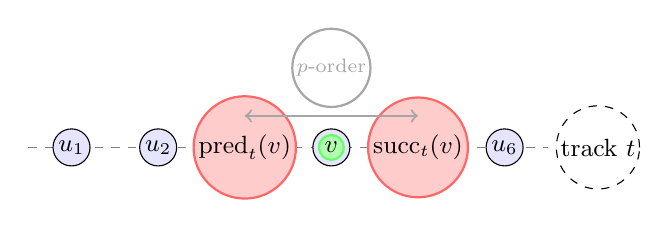
\begin{tikzpicture}[x=1.1cm,y=1cm,
    every node/.style={circle,draw,inner sep=1pt,font=\small}]
    % Single track line
    \draw[dashed,gray] (0.5,0) -- (6.5,0)
      node[right=1mm,black] {$\text{track }t$};

    % Vertices on track t
    \foreach \i in {1,...,6} {
      \node[fill=blue!10] (u\i) at (\i,0) {$u_{\i}$};
    }

    % Highlight v = u4
    \node[fill=green!30,draw=green!60,thick] (v) at (4,0) {$v$};

    % Overwrite labels for pred and succ
    \node[fill=red!20,draw=red!60,thick] (pred) at (3,0)
      {$\operatorname{pred}_t(v)$};
    \node[fill=red!20,draw=red!60,thick] (succ) at (5,0)
      {$\operatorname{succ}_t(v)$};

    % Order indication
    \draw[<->,thick,gray!70] (3,0.4) -- node[above=1mm,font=\scriptsize]
      {$p$-order} (5,0.4);
  \end{tikzpicture}
  \caption{Predecesor y sucesor de un vértice $v$ en un track $t$ en el orden global.}
  \label{fig:predsucc}
\end{figure}


\begin{definition}[Conjunto de vecinos legales y grafo anfitrión]
Dado $(\tau,p)$, el \emph{conjunto de vecinos legales} de $v\in V$ es
\[
  N_{\mathrm{legal}}(v)
  :=
  \bigl\{\operatorname{pred}_t(v), \operatorname{succ}_t(v)
        : t=1,\dots,k\bigr\}\setminus\{\text{inexistente}\}.
\]
El \emph{grafo anfitrión} correspondiente $H(\tau,p)$ sobre el conjunto de
vértices $V$ tiene conjunto de aristas
\[
  E\bigl(H(\tau,p)\bigr)
  :=
  \bigl\{\{u,v\} : u\in N_{\mathrm{legal}}(v)\bigr\}.
\]
\end{definition}
La Figura~\ref{fig:legal-neighbors} muestra $N_{\mathrm{legal}}(v)$ en tres tracks.

\begin{figure}[ht]
  \centering
  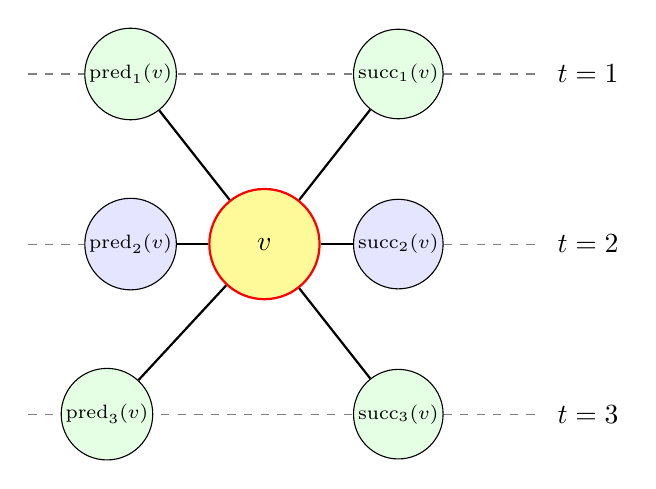
\begin{tikzpicture}[x=1.0cm,y=1.2cm,  % increased vertical spacing
    neighbor/.style={
      circle,draw,
      minimum size=10mm,  % smaller nodes
      font=\scriptsize,
      inner sep=1pt
    },
    central/.style={
      circle,draw,
      minimum size=14mm,  % central node larger
      font=\normalsize,
      inner sep=2pt,
      fill=yellow!40,
      draw=red,
      thick
    }
  ]

    % Track lines (shift y more apart so circles don't touch)
    \foreach \t/\y in {1/1.8,2/0.0,3/-1.8} {
      \draw[dashed,gray] (0.5,\y) -- (7.0,\y)
        node[right=1mm,black] {$t=\t$};
    }

    % Central vertex v
    \node[central] (v) at (3.5,0.0) {$v$};

    % Track 1 neighbors
    \node[neighbor,fill=green!10] (p1) at (1.8,1.8)
      {$\operatorname{pred}_1(v)$};
    \node[neighbor,fill=green!10] (s1) at (5.2,1.8)
      {$\operatorname{succ}_1(v)$};

    % Track 2 neighbors
    \node[neighbor,fill=blue!10] (p2) at (1.8,0.0)
      {$\operatorname{pred}_2(v)$};
    \node[neighbor,fill=blue!10] (s2) at (5.2,0.0)
      {$\operatorname{succ}_2(v)$};

    % Track 3 neighbors
    \node[neighbor,fill=green!10] (p3) at (1.5,-1.8)
      {$\operatorname{pred}_3(v)$};
    \node[neighbor,fill=green!10] (s3) at (5.2,-1.8)
      {$\operatorname{succ}_3(v)$};

    % Edges
    \foreach \w in {p1,s1,p2,s2,p3,s3} {
      \draw[thick] (v) -- (\w);
    }

  \end{tikzpicture}
  \caption{El conjunto de vecinos legales $N_{\mathrm{legal}}(v)$.}
  \label{fig:legal-neighbors}

\end{figure}



\begin{definition}[Grafo representable por vecinos más cercanos en $k$ tracks]
Un grafo $G=(V,E)$ es \emph{representable por vecinos más cercanos en $k$ tracks}
si existe un diseño ordenado en $k$ tracks $(\tau,p)$ de $V$ tal que
\[
  E \subseteq E\bigl(H(\tau,p)\bigr),
\]
es decir, cada arista de $G$ es una arista legal en el grafo anfitrión.
Equivalentemente,
\[
  \forall v\in V,\quad N_G(v) \subseteq N_{\mathrm{legal}}(v).
\]
El menor $k$ con esta propiedad (si existe) es el \emph{número de tracks de
vecinos más cercanos} de $G$.
\end{definition}
La Figura~\ref{fig:k1-linear-forest} ilustra un grafo anfitrión típico
cuando $k=1$. La Figura~\ref{fig:k2-host-example} muestra un grafo anfitrión
típico cuando $k=2$.


\begin{figure}[ht]
  \centering
  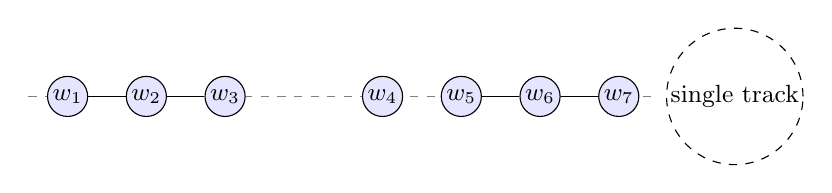
\begin{tikzpicture}[x=1cm,y=1cm,
    every node/.style={circle,draw,inner sep=1pt,font=\small}]
    % Single track
    \draw[dashed,gray] (0.5,0) -- (8.5,0)
      node[right=1mm,black] {$\text{single track}$};

    % Vertices in global order
    \foreach \i/\x in {1/1,2/2,3/3,4/5,5/6,6/7,7/8} {
      \node[fill=blue!10] (w\i) at (\x,0) {$w_{\i}$};
    }

    % Path components: w1-w2-w3 and w5-w6-w7; w4 isolated
    \draw (w1) -- (w2) -- (w3);
    \draw (w5) -- (w6) -- (w7);
  \end{tikzpicture}
  \caption{Con un solo track, el grafo anfitrión es una unión disjunta de caminos y vértices aislados (un bosque lineal).}
  \label{fig:k1-linear-forest}
\end{figure}

\begin{figure}[ht]
  \centering
  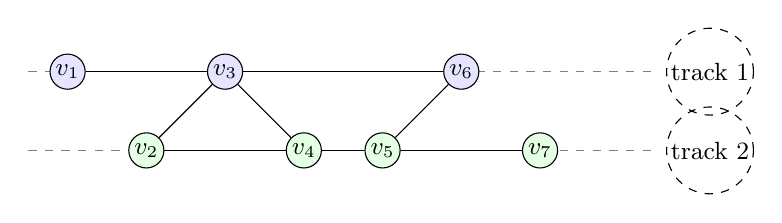
\begin{tikzpicture}[x=1cm,y=1cm,
    every node/.style={circle,draw,inner sep=1pt,font=\small}]
    % Two tracks
    \draw[dashed,gray] (0.5,1) -- (8.5,1)
      node[right=1mm,black] {$\text{track }1$};
    \draw[dashed,gray] (0.5,0) -- (8.5,0)
      node[right=1mm,black] {$\text{track }2$};

    % Vertices in global order v1,...,v7
    % Track 1: v1, v3, v6
    \node[fill=blue!10]  (v1) at (1,1) {$v_1$};
    \node[fill=blue!10]  (v3) at (3,1) {$v_3$};
    \node[fill=blue!10]  (v6) at (6,1) {$v_6$};

    % Track 2: v2, v4, v5, v7
    \node[fill=green!10] (v2) at (2,0) {$v_2$};
    \node[fill=green!10] (v4) at (4,0) {$v_4$};
    \node[fill=green!10] (v5) at (5,0) {$v_5$};
    \node[fill=green!10] (v7) at (7,0) {$v_7$};

    % Same-track edges: nearest neighbors along each track
    % Track 1 path
    \draw (v1) -- (v3) -- (v6);
    % Track 2 path
    \draw (v2) -- (v4) -- (v5) -- (v7);

    % Cross-track edges between nearest opposite-track neighbors
    \draw (v3) -- (v2);
    \draw (v3) -- (v4);
    \draw (v5) -- (v6);

  \end{tikzpicture}
  \caption{Con dos tracks, el grafo anfitrión puede tener tramos tipo camino en cada track más aristas cruzadas entre vecinos más cercanos en el otro track.}
  \label{fig:k2-host-example}
\end{figure}


\begin{remark}[Qué significa realmente $k=1$]
\label{rem:what-k1-means}
Cuando $k=1$, todo vértice tiene a lo sumo un predecesor y un sucesor,
de modo que el grafo anfitrión $H(\tau,p)$ es un subgrafo de un camino
simple. Entonces cualquier grafo representable por vecinos más cercanos
en un solo track es una unión disjunta de caminos y vértices aislados
(un \emph{bosque lineal}). Esto va a ser importante cuando discutamos
cuándo es posible ``menos de dos colores'' (tracks).
\end{remark}

\begin{remark}[Qué significa realmente $k=2$]
\label{rem:what-k2-means}

Cuando $k=2$, cada vértice puede tener a lo sumo dos vecinos legales en su
propio track (un predecesor y un sucesor) y a lo sumo dos vecinos legales
en el otro track (de nuevo, un predecesor y un sucesor allí). Entonces
cada vértice en el grafo anfitrión $H(\tau,p)$ tiene grado a lo sumo $4$,
y $H(\tau,p)$ se puede ver como dos capas tipo camino (una por track) con
aristas cruzadas adicionales entre vecinos más cercanos de la otra capa,
como en la Figura~\ref{fig:k2-host-example}. En particular, cualquier
grafo representable por vecinos más cercanos en $2$ tracks es un subgrafo
de un grafo anfitrión planar de este tipo ``escalera''. Esto será importante
cuando discutamos cuándo es posible ``menos de tres colores'' (tracks).
\end{remark}

% =====================================================
\section{De patrones coloreados prohibidos a restricciones en tríos}
% =====================================================

La formulación del Investigathon usa patrones \emph{coloreados} prohibidos
sobre triples de vértices. Ahora traducimos ese lenguaje a nuestro setting
de diseños en $k$ tracks.

\subsection{Patrones coloreados en triples}

\begin{definition}[Patrón coloreado en tres vértices]
Fijamos el conjunto de índices $\{1,2,3\}$. Un \emph{patrón} (a secas) es un par
\[
  (E_P, N_P),
\]
donde $E_P, N_P \subseteq \{1,2,3\} \times \{1,2,3\}$ codifican aristas que
deben estar presentes y aristas que deben estar ausentes entre las tres
posiciones distinguidas.

Un \emph{patrón coloreado} es un triple
\[
  P = (E_P, N_P, C_P),
\]
donde $(E_P, N_P)$ es un patrón como antes y
$C_P \subseteq \{1,2,3\}$ es el conjunto de índices que deben quedar en
una misma clase de color.
\end{definition}

En el setting del Investigathon, el input es:
\begin{itemize}[leftmargin=2em]
  \item un orden lineal $<$ sobre $V(G)$, y
  \item una partición (``coloración'')
    $\mathcal{S} = \{S_1,\dots,S_k\}$ de $V(G)$ en $k$ clases de color.
\end{itemize}

\begin{definition}[Realizar un patrón coloreado]
Dados $(\mathcal{S},<)$ como arriba y un patrón coloreado
$P = (E_P,N_P,C_P)$, un triple ordenado de vértices distintos
\[
  v_1 < v_2 < v_3
\]
\emph{realiza} $P$ si:
\begin{enumerate}[label=(\roman*), leftmargin=2em]
  \item para todo $(i,j)\in E_P$ se cumple $\{v_i,v_j\}\in E(G)$;
  \item para todo $(i,j)\in N_P$ se cumple $\{v_i,v_j\}\notin E(G)$;
  \item todos los $v_i$ con $i\in C_P$ pertenecen a una misma clase de color
        en $\mathcal{S}$.
\end{enumerate}
Decimos que $(\mathcal{S},<)$ \emph{evita} $P$ si no hay ningún triple
$v_1<v_2<v_3$ que realice $P$.
\end{definition}

Dada una familia finita $\Pi$ de patrones coloreados, $(\mathcal{S},<)$
\emph{evita $\Pi$} si evita a cada $P\in\Pi$.

\subsection{Los patrones del Investigathon}

En nuestro caso, la familia prohibida $\Pi$ consiste en dos patrones:
\begin{align*}
  P^{(1)} &: \quad
    E_{P^{(1)}} = \{(1,3)\},\quad
    N_{P^{(1)}} = \varnothing,\quad
    C_{P^{(1)}} = \{1,2\},\\[0.3em]
  P^{(2)} &: \quad
    E_{P^{(2)}} = \{(1,3)\},\quad
    N_{P^{(2)}} = \varnothing,\quad
    C_{P^{(2)}} = \{2,3\}.
\end{align*}
Intuitivamente:
\begin{itemize}[leftmargin=2em]
  \item $P^{(1)}$ prohíbe triples $x<y<z$ con $\{x,z\}\in E(G)$ y $x,y$
        del mismo color;
  \item $P^{(2)}$ prohíbe triples $x<y<z$ con $\{x,z\}\in E(G)$ y $y,z$
        del mismo color.
\end{itemize}
Ver Figuras~\ref{fig:pattern-P1} y~\ref{fig:pattern-P2}.
\begin{figure}[ht]
  \centering
  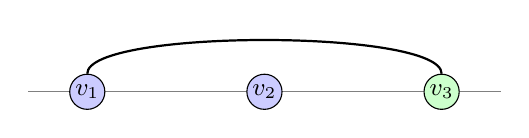
\begin{tikzpicture}[x=1.5cm,y=1cm,
    every node/.style={circle,draw,inner sep=1pt,font=\small}]
    % Order line
    \draw[gray] (0.5,0) -- (4.5,0);

    % Vertices v1 < v2 < v3
    \node[fill=blue!20]  (v1) at (1,0) {$v_1$};
    \node[fill=blue!20]  (v2) at (2.5,0) {$v_2$};
    \node[fill=green!20] (v3) at (4,0) {$v_3$};

    % Edge {v1,v3}
    \draw[thick] (v1) .. controls +(0,0.8) and +(0,0.8) .. (v3);


  \end{tikzpicture}
  \caption{Patrón prohibido $P^{(1)}$: $v_1<v_2<v_3$ con $\{v_1,v_3\}\in E(G)$ y $v_1,v_2$ en la misma clase de color.}
  \label{fig:pattern-P1}
\end{figure}
\begin{figure}[ht]
  \centering
  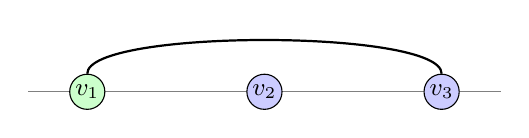
\begin{tikzpicture}[x=1.5cm,y=1cm,
    every node/.style={circle,draw,inner sep=1pt,font=\small}]
    % Order line
    \draw[gray] (0.5,0) -- (4.5,0);

    % Vertices v1 < v2 < v3
    \node[fill=green!20] (v1) at (1,0) {$v_1$};
    \node[fill=blue!20]  (v2) at (2.5,0) {$v_2$};
    \node[fill=blue!20]  (v3) at (4,0) {$v_3$};

    % Edge {v1,v3}
    \draw[thick] (v1) .. controls +(0,0.8) and +(0,0.8) .. (v3);


  \end{tikzpicture}
  \caption{Patrón prohibido $P^{(2)}$: $v_1<v_2<v_3$ con $\{v_1,v_3\}\in E(G)$ y $v_2,v_3$ en la misma clase de color.}
  \label{fig:pattern-P2}
\end{figure}

Una \emph{solución con a lo sumo $k$ colores} en el sentido del Investigathon
es exactamente un par $(\mathcal{S},<)$ con $|\mathcal{S}|\le k$ que evita
$P^{(1)}$ y $P^{(2)}$.

\subsection{Tracks como clases de color}

Dado un diseño en $k$ tracks $(\tau,p)$, la asignación de tracks induce una
partición en clases de color
\[
  S_i := \{ v\in V(G) : \tau(v) = i \},
  \qquad \mathcal{S} = \{S_1,\dots,S_k\},
\]
y el orden global $<$ está definido por $p$.

A la inversa, dada una partición $\mathcal{S} = \{S_1,\dots,S_k\}$ y un
orden lineal $<$, obtenemos un diseño en $k$ tracks etiquetando las partes
$S_1,\dots,S_k$ y fijando $\tau(v)=i$ para $v\in S_i$, y tomando un $p$
cualquiera biyección compatible con $<$.

Así, hay una correspondencia uno a uno entre:
\begin{itemize}[leftmargin=2em]
  \item soluciones $(\mathcal{S},<)$ con a lo sumo $k$ colores, y
  \item diseños ordenados en $k$ tracks $(\tau,p)$.
\end{itemize}

\subsection{Formulación como restricción en tríos}

Reexpresamos ahora la evitación de $P^{(1)}$ y $P^{(2)}$ de forma compacta.

\begin{lemma}[Patrones coloreados vs.\ restricción de tríos]
\label{lem:patterns-triplet-equivalence}
Sea $G=(V,E)$ un grafo y sea $(\tau,p)$ un diseño ordenado en $k$ tracks
con el orden asociado $<$ y la partición inducida $\mathcal{S}$ como arriba.
Entonces son equivalentes:
\begin{enumerate}[label=(\arabic*), leftmargin=2em]
  \item $(\mathcal{S},<)$ evita ambos patrones coloreados $P^{(1)}$ y $P^{(2)}$.
  \item Para todo trío $x,y,z\in V$ con
        \[
          p(x) < p(y) < p(z)
          \quad\text{y}\quad
          \{x,z\}\in E(G),
        \]
        se cumple
        \[
          \tau(y) \neq \tau(x)
          \quad\text{y}\quad
          \tau(y) \neq \tau(z).
        \]
\end{enumerate}
\end{lemma}

\begin{proof}
$(1)\Rightarrow(2)$:
Supongamos que existen $x,y,z$ con $p(x)<p(y)<p(z)$ y $\{x,z\}\in E(G)$
tales que $\tau(y)=\tau(x)$ o $\tau(y)=\tau(z)$.

Escribimos $v_1:=x$, $v_2:=y$, $v_3:=z$. Entonces $\{v_1,v_3\}\in E(G)$.
Si $\tau(y)=\tau(x)$, entonces $v_1$ y $v_2$ están en la misma clase de
color y el trío $(v_1,v_2,v_3)$ realiza $P^{(1)}$, contradiciendo que se
evita $P^{(1)}$. Si $\tau(y)=\tau(z)$, entonces $(v_1,v_2,v_3)$ realiza
$P^{(2)}$, otra contradicción. Por lo tanto, $\tau(y)$ es distinto tanto
de $\tau(x)$ como de $\tau(z)$.

\medskip
$(2)\Rightarrow(1)$:
Asumamos que vale (2). Supongamos que algún triple $v_1<v_2<v_3$ realiza
$P^{(1)}$. Entonces $\{v_1,v_3\}\in E(G)$ y $v_1,v_2$ están en la misma
clase de color, o sea $\tau(v_1)=\tau(v_2)$, lo que contradice (2) con
$(x,y,z)=(v_1,v_2,v_3)$. Un argumento idéntico, permutando los roles de
las posiciones $\{1,2\}$ y $\{2,3\}$, muestra que ningún triple realiza
$P^{(2)}$ tampoco.
\end{proof}

\begin{definition}[Diseño triplemente-legal en $k$ tracks]
Un diseño ordenado en $k$ tracks $(\tau,p)$ de $G$ es \emph{triplemente-legal}
si para todo $x,y,z\in V$ con
\[
  p(x) < p(y) < p(z) \quad\text{y}\quad \{x,z\}\in E(G),
\]
se cumple
\[
  \tau(y) \neq \tau(x)
  \quad\text{y}\quad
  \tau(y) \neq \tau(z).
\]
Por el Lema~\ref{lem:patterns-triplet-equivalence}, los diseños
triplemente-legales son exactamente los diseños que corresponden a soluciones
del Investigathon que evitan $P^{(1)}$ y $P^{(2)}$.
\end{definition}
La Figura~\ref{fig:triplet-legal} contrasta un triple prohibido y dos triples
legales, uno usando menos colores que el otro.
\begin{figure}[ht]
  \centering
  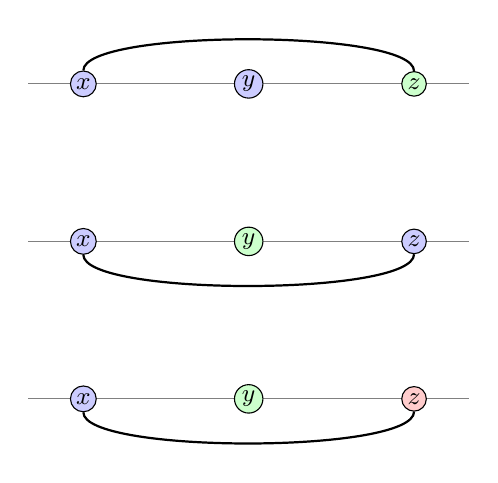
\begin{tikzpicture}[x=1.4cm,y=1cm,
    every node/.style={circle,draw,inner sep=1pt,font=\small}]

    % Forbidden triple (top)
    \draw[gray] (0.5,0.8) -- (4.5,0.8);
    \node[fill=blue!20]  (x1) at (1,0.8) {$x$};
    \node[fill=blue!20]  (y1) at (2.5,0.8) {$y$};
    \node[fill=green!20] (z1) at (4,0.8) {$z$};
    \draw[thick] (x1) .. controls +(0,0.7) and +(0,0.7) .. (z1);

    % Legal triple (bottom)
    \draw[gray] (0.5,-1.2) -- (4.5,-1.2);
    \node[fill=blue!20]  (x2) at (1,-1.2) {$x$};
    \node[fill=green!20] (y2) at (2.5,-1.2) {$y$};
    \node[fill=blue!20]   (z2) at (4,-1.2) {$z$};
    \draw[thick] (x2) .. controls +(0,-0.7) and +(0,-0.7) .. (z2);

    \draw[gray] (0.5,-3.2) -- (4.5,-3.2);
    \node[fill=blue!20]  (x3) at (1,-3.2) {$x$};
    \node[fill=green!20] (y3) at (2.5,-3.2) {$y$};
    \node[fill=red!20]   (z3) at (4,-3.2) {$z$};
    \draw[thick] (x3) .. controls +(0,-0.7) and +(0,-0.7) .. (z3);
  \end{tikzpicture}
  \caption{Arriba: un triple prohibido donde $y$ comparte track (color) con $x$. 
  Medio: un triple legal donde $x$ comparte track (color) con $z$. 
  Abajo: un triple legal donde el vértice del medio está en un tercer track.}
  \label{fig:triplet-legal}
\end{figure}

\begin{remark}[Vecinos más cercanos vs.\ triplemente-legal]
La representabilidad por vecinos más cercanos es una condición
\emph{más fuerte} que ser triplemente-legal: en un diseño por vecinos
más cercanos, cada arista debe ser entre vecinos más cercanos en algún track;
en un diseño triplemente-legal sólo prohibimos ciertos patrones coloreados
en triples. En la próxima sección mostramos que los diseños de vecinos más
cercanos satisfacen automáticamente la restricción de tríos.
\end{remark}
% =====================================================
\section{Número cromático vs.\ ``colores'' basados en tracks}
% =====================================================

El índice de track $\tau(v)$ se comporta un poco como un color, pero
\emph{no} es una coloración propia en el sentido clásico (se permiten aristas
dentro de un mismo track). Sólo necesitaremos dos hechos estándar del
colorido clásico para la analogía:

\begin{itemize}[leftmargin=2em]
  \item Si $G_1,\dots,G_r$ son las componentes conexas de $G$, entonces
        \[
          \chi(G) \;=\; \max_{1\le i\le r} \chi(G_i).
        \]
  \item Si $G$ contiene un clique de tamaño $r$, entonces $\chi(G)\ge r$;
        en particular un $K_4$ fuerza al menos cuatro colores.
\end{itemize}

En el setting de vecinos más cercanos, las etiquetas de track juegan el rol
de ``colores'', y vamos a ver análogos de ambas afirmaciones para el número
de tracks.

\subsection{Número de tracks y componentes conexas}

\begin{definition}[Número de tracks de vecinos más cercanos]
El \emph{número de tracks de vecinos más cercanos} de un grafo $G$,
denotado por $\operatorname{tn}(G)$, es el mínimo $k\in\mathbb{N}$ tal
que $G$ es representable por vecinos más cercanos en $k$ tracks.
\end{definition}

\begin{proposition}[Número de tracks y componentes conexas]
\label{prop:tracknumber-components}
Sean $G_1,\dots,G_r$ las componentes conexas de $G$. Entonces
\[
  \operatorname{tn}(G)
  \;=\;
  \max_{1\le i\le r} \operatorname{tn}(G_i).
\]
\end{proposition}
\begin{remark}
La Proposición~\ref{prop:tracknumber-components} es directamente análoga al
hecho clásico de que $\chi(G) = \max_i \chi(G_i)$ para el número cromático:
en ambos settings, la cantidad de ``colores'' que se necesitan para todo el
grafo es el máximo sobre sus componentes conexas.
\end{remark}

\begin{proof}
\emph{Cota inferior.}
Cualquier diseño que prueba que $G$ es representable por vecinos más cercanos
en $k$ tracks se restringe a un diseño para cada $G_i$, de modo que
$\operatorname{tn}(G_i)\le k$. Tomando el mínimo sobre todos esos $k$ se
obtiene
\(
  \max_i \operatorname{tn}(G_i) \le \operatorname{tn}(G).
\)

\smallskip
\noindent\emph{Cota superior.}
Sea $k_i = \operatorname{tn}(G_i)$ y $k:=\max_i k_i$. Para cada componente
$G_i$ elegimos un diseño en $k_i$ tracks $(\tau_i,p_i)$ que pruebe la
representabilidad por vecinos más cercanos. Renombramos los tracks de forma
que $\tau_i$ tome valores en $\{1,\dots,k\}$ (simplemente no usamos todos
los labels cuando $k_i<k$).

Ahora ponemos las componentes una detrás de la otra en el orden global:
definimos $p$ apilando los órdenes $p_1,\dots,p_r$ con rangos disjuntos,
y fijamos $\tau(v)=\tau_i(v)$ para $v\in V(G_i)$. Esto da un diseño en
$k$ tracks $(\tau,p)$ de $G$ en el que cada arista dentro de cada componente
sigue siendo legal. No hay aristas entre componentes, así que no hay nada
más que chequear. Por lo tanto, $G$ es representable por vecinos más
cercanos en $k$ tracks y $\operatorname{tn}(G)\le k$.
\end{proof}

La Figura~\ref{fig:tn-components} muestra cómo los diseños de tracks para
componentes diferentes se pueden apilar en el orden global reutilizando
el mismo conjunto de labels de track.

\begin{figure}[ht]
  \centering
  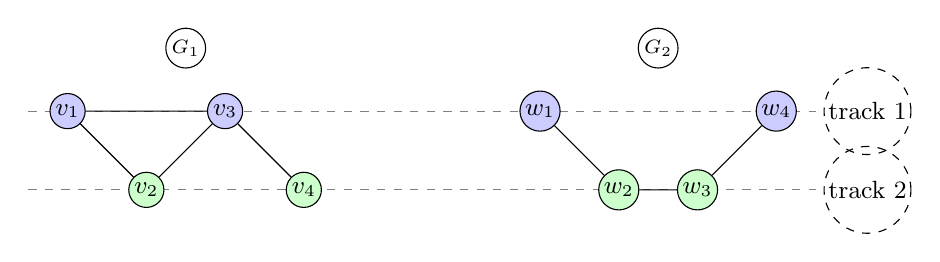
\begin{tikzpicture}[x=1.0cm,y=1cm,
    every node/.style={circle,draw,inner sep=1pt,font=\small}]

    % Track lines
    \foreach \t/\y in {1/1.0,2/0.0} {
      \draw[dashed,gray] (0.5,\y) -- (10.5,\y)
        node[right=1mm,black] {$\text{track }\t$};
    }

    % Component G1 on the left (vertices v1..v4)
    \node[fill=blue!20] (v1) at (1,1.0) {$v_1$};
    \node[fill=green!20] (v2) at (2,0.0) {$v_2$};
    \node[fill=blue!20] (v3) at (3,1.0) {$v_3$};
    \node[fill=green!20] (v4) at (4,0.0) {$v_4$};
    \draw (v1) -- (v2) -- (v3) -- (v4) -- (v3) -- (v1);

    % Component G2 on the right (vertices w1..w4)
    \node[fill=blue!20] (w1) at (7,1.0) {$w_1$};
    \node[fill=green!20] (w2) at (8,0.0) {$w_2$};
    \node[fill=green!20] (w3) at (9,0.0) {$w_3$};
    \node[fill=blue!20] (w4) at (10,1.0) {$w_4$};
    \draw (w1) -- (w2) -- (w3) -- (w4);

    \node at (2.5,1.8) {\scriptsize $G_1$};
    \node at (8.5,1.8) {\scriptsize $G_2$};
  \end{tikzpicture}
  \caption{Los diseños para distintas componentes comparten los mismos labels
  de track. El orden global apila las componentes una tras otra.}
  \label{fig:tn-components}
\end{figure}

\begin{remark}[Cuándo alcanza con menos de $2$ tracks]
De la Sección~\ref{sec:basic-setup}, un grafo anfitrión con $1$ track es
siempre una unión disjunta de caminos y vértices aislados (un bosque lineal).
Entonces
\[
  \operatorname{tn}(G)=1 \quad\Longleftrightarrow\quad
  G \text{ es un bosque lineal},
\]
y todo grafo que contenga un ciclo requiere al menos dos tracks. La
Figura~\ref{fig:cycle-needs-two} ilustra por qué un ciclo no puede vivir
en un solo track.
\end{remark}

\begin{figure}[ht]
  \centering
  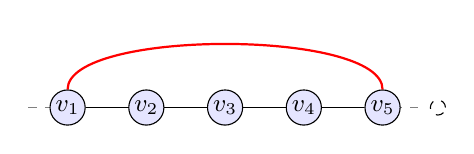
\begin{tikzpicture}[x=1cm,y=1cm,
    every node/.style={circle,draw,inner sep=1pt,font=\small}]

    % Single track
    \draw[dashed,gray] (0.5,0) -- (5.5,0)
      node[right=1mm,black] {$\text{ }$};

    % Vertices in order v1..v5
    \foreach \i/\x in {1/1,2/2,3/3,4/4,5/5} {
      \node[fill=blue!10] (v\i) at (\x,0) {$v_{\i}$};
    }

    % Path edges (legal)
    \draw (v1) -- (v2) -- (v3) -- (v4) -- (v5);

    % Extra edge v5-v1 (would form a cycle)
    \draw[thick,red] (v1) .. controls +(0,1) and +(0,1) .. (v5);

  \end{tikzpicture}
  \caption{En un solo track sólo pueden ser legales aristas entre vértices
  consecutivos. La arista $\{v_1,v_5\}$ necesaria para completar un ciclo
  salta tres vértices y no se puede realizar.}
  \label{fig:cycle-needs-two}
\end{figure}

% =====================================================
\section{Los diseños de vecinos más cercanos cumplen la restricción de tríos}
% =====================================================

Ahora conectamos la condición de vecinos más cercanos con la restricción
de tríos del Lema~\ref{lem:patterns-triplet-equivalence}.

\begin{lemma}[Restricción de tríos para diseños de vecinos más cercanos]
\label{lem:triplet}
Sea $(\tau,p)$ un diseño ordenado en $k$ tracks de un grafo $G=(V,E)$ y
supongamos que $G$ es representable por vecinos más cercanos en $k$ tracks
respecto de $(\tau,p)$, es decir
\[
  N_G(v) \subseteq N_{\mathrm{legal}}(v)
  \quad\text{para todo }v\in V.
\]
Sean $x,y,z\in V$ tales que
\[
  p(x) < p(y) < p(z),
\]
y supongamos que $\{x,z\}\in E$. Entonces
\[
  \tau(y) \neq \tau(x)
  \quad\text{y}\quad
  \tau(y) \neq \tau(z).
\]
En palabras: cualquier vértice estrictamente entre $x$ y $z$ en el orden
global debe estar en un track distinto tanto de $\tau(x)$ como de $\tau(z)$.
\end{lemma}
La Figura~\ref{fig:triplet-lemma} muestra la situación del Lema~\ref{lem:triplet}.

\begin{figure}[ht]
  \centering
  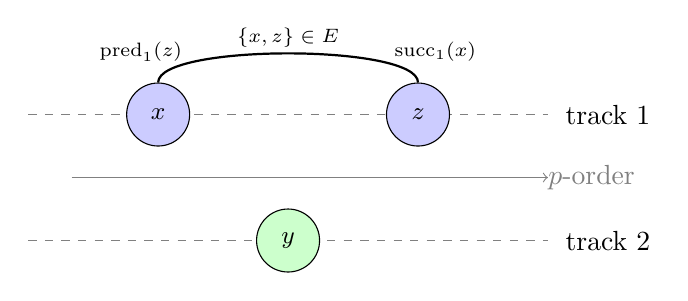
\begin{tikzpicture}[
    x=1.1cm,y=1cm,
    vertex/.style={circle,draw,inner sep=1pt,minimum size=8mm,font=\small}
  ]

    % Two tracks
    \draw[dashed,gray] (0.5,0.8) -- (6.5,0.8)
      node[right=1mm,black] {$\text{track }1$};
    \draw[dashed,gray] (0.5,-0.8) -- (6.5,-0.8)
      node[right=1mm,black] {$\text{track }2$};

    % x and z on track 1, y on track 2 (bigger vertices)
    \node[vertex,fill=blue!20] (x) at (2,0.8) {$x$};
    \node[vertex,fill=blue!20] (z) at (5,0.8) {$z$};
    \node[vertex,fill=green!20] (y) at (3.5,-0.8) {$y$};

    % Global order on the x-axis
    \draw[->,gray] (1,0) -- (6.5,0)
      node[right,draw=none,inner sep=0] {$p$-order};

    % Edge between x and z
    \draw[thick] (x) .. controls +(0,0.9) and +(0,0.9) .. (z);
    \node[above=7mm,draw=none,inner sep=0] at (3.5,0.95)
      {\scriptsize $\{x,z\}\in E$};

    % Nearest neighbors of x and z on track 1 (no circles)
    \node[draw=none,inner sep=0,font=\scriptsize] at (1.8,1.6)
      {$\operatorname{pred}_1(z)$};
    \node[draw=none,inner sep=0,font=\scriptsize] at (5.2,1.6)
      {$\operatorname{succ}_1(x)$};

  \end{tikzpicture}
  \caption{Si $\{x,z\}$ es una arista que viene de vecinos más cercanos en el track~1, entonces no puede haber otro vértice en el track~1 entre ellos en el orden global. Por lo tanto cualquier vértice del medio $y$ debe vivir en otro track.}
  \label{fig:triplet-lemma}
\end{figure}


\begin{proof}
Como $\{x,z\}\in E$ y $G$ es representable por vecinos más cercanos, tenemos
\[
  z \in N_{\mathrm{legal}}(x)
  \quad\text{y}\quad
  x \in N_{\mathrm{legal}}(z).
\]

\medskip
\noindent\emph{Paso 1: $z$ es el sucesor de $x$ en el track $\tau(z)$.}

Por definición de $N_{\mathrm{legal}}(x)$, existe un track $t$ tal que
\[
  z = \operatorname{pred}_t(x)
  \quad\text{o}\quad
  z = \operatorname{succ}_t(x).
\]
Si $z = \operatorname{pred}_t(x)$ entonces $p(z)<p(x)$, contradiciendo
$p(x)<p(z)$; luego
\[
  z = \operatorname{succ}_t(x).
\]
Además, $\operatorname{succ}_t(x)$ está en el track $t$, así que
$\tau(z)=t$ y
\[
  z = \operatorname{succ}_{\tau(z)}(x).
\]

Por definición de sucesor, no hay vértices $w$ en el track $\tau(z)$
con posición global estrictamente entre $p(x)$ y $p(z)$, es decir
\[
  \text{no hay }w\text{ tal que }\tau(w)=\tau(z)\text{ y }p(x)<p(w)<p(z).
\]
Como $p(x)<p(y)<p(z)$, no puede pasar que $\tau(y)=\tau(z)$.

\medskip
\noindent\emph{Paso 2: $x$ es el predecesor de $z$ en el track $\tau(x)$.}

Análogamente, como $x\in N_{\mathrm{legal}}(z)$ existe un track $s$ tal que
\[
  x = \operatorname{pred}_s(z)
  \quad\text{o}\quad
  x = \operatorname{succ}_s(z).
\]
Como $p(x)<p(z)$, $x$ no puede ser sucesor de $z$, así que
\[
  x = \operatorname{pred}_s(z).
\]
Luego $\tau(x)=s$ y
\[
  x = \operatorname{pred}_{\tau(x)}(z).
\]
De nuevo por definición de predecesor, no hay vértices $w$ en el track
$\tau(x)$ con $p(x)<p(w)<p(z)$. En particular, $\tau(y)\neq \tau(x)$.

\medskip
Combinando ambos pasos, obtenemos $\tau(y)\neq\tau(x)$ y
$\tau(y)\neq\tau(z)$.
\end{proof}

\begin{corollary}
Todo diseño de vecinos más cercanos en $k$ tracks $(\tau,p)$ es un diseño
triplemente-legal en $k$ tracks. En particular, cualquier solución de
vecinos más cercanos evita automáticamente los patrones del Investigathon
$P^{(1)}$ y $P^{(2)}$.
\end{corollary}

\begin{proof}
Aplicar el Lema~\ref{lem:triplet} y luego el
Lema~\ref{lem:patterns-triplet-equivalence}.
\end{proof}

% =====================================================
\section{Cotas de grado y restricciones de cliques}
% =====================================================

Ahora cuantificamos cómo el número de tracks $k$ controla los posibles grados
y cliques en un grafo representable por vecinos más cercanos. Esto apunta
a una forma natural de \emph{acotar por abajo} la cantidad de ``colores''
(tracks) necesarios.

\subsection{Un $K_4$ fuerza al menos tres tracks}

\begin{theorem}[Un clique de tamaño $4$ fuerza $k\ge 3$]
\label{thm:K4-needs-3}
Sea $G=(V,E)$ un grafo representable por vecinos más cercanos en $k$ tracks
para algún $k\in\mathbb{N}$. Si $G$ contiene un clique de tamaño $4$, entonces
$k \ge 3$. Equivalentemente, ningún diseño en $1$ o $2$ tracks puede
representar un $4$-clique.
\end{theorem}

\begin{proof}
Sea $H\subseteq G$ un subgrafo isomorfo a $K_4$ con conjunto de vértices
$\{a,b,c,d\}$. Sea $(\tau,p)$ un diseño ordenado en $k$ tracks que pruebe
la representabilidad por vecinos más cercanos de $G$.

Renombramos $a,b,c,d$ de forma que
\[
  p(a) < p(b) < p(c) < p(d).
\]
Como $H$ es completo, cada par entre $\{a,b,c,d\}$ es una arista.

Usando el Lema~\ref{lem:triplet}, aplicamos la restricción de tríos a todos
los triples $(x,y,z)$ con $x<y<z$ donde $\{x,z\}$ es una arista (siempre
cierto en $K_4$). Los triples relevantes y sus consecuencias son:
\begin{align}
\tau(b) &\neq \tau(a), \quad \tau(b) \neq \tau(c),
   &&\text{a partir de }(a,b,c)\text{ y la arista }\{a,c\}, \label{eq:bc1}\\
\tau(b) &\neq \tau(a), \quad \tau(b) \neq \tau(d),
   &&\text{a partir de }(a,b,d)\text{ y la arista }\{a,d\}, \label{eq:bd1}\\
\tau(c) &\neq \tau(a), \quad \tau(c) \neq \tau(d),
   &&\text{a partir de }(a,c,d)\text{ y la arista }\{a,d\}, \label{eq:cd1}\\
\tau(c) &\neq \tau(b), \quad \tau(c) \neq \tau(d),
   &&\text{a partir de }(b,c,d)\text{ y la arista }\{b,d\}. \label{eq:cd2}
\end{align}
De \eqref{eq:bc1} y \eqref{eq:bd1} vemos que
\[
  \tau(b) \notin \{\tau(a),\tau(c),\tau(d)\},
\]
y de \eqref{eq:cd1} y \eqref{eq:cd2} que
\[
  \tau(c) \notin \{\tau(a),\tau(b),\tau(d)\}.
\]

Supongamos $k\le 2$. Entonces los tracks son $\{1,2\}$.
Sin pérdida de generalidad, tomemos $\tau(a)=1$.

\smallskip
\noindent\emph{Caso 1: $\tau(d)=1$.}
Entonces \eqref{eq:bd1} implica $\tau(b)\neq \tau(a)$ y $\tau(b)\neq \tau(d)$,
así que $\tau(b)\neq 1$ y por lo tanto $\tau(b)=2$. Análogamente,
\eqref{eq:cd1} implica $\tau(c)\neq 1$, luego $\tau(c)=2$. Pero entonces
\eqref{eq:bc1} exige $\tau(b)\neq \tau(c)$, imposible.

\smallskip
\noindent\emph{Caso 2: $\tau(d)=2$.}
Entonces \eqref{eq:bd1} dice que $\tau(b)\neq 1$ y $\tau(b)\neq 2$, lo cual
es imposible con sólo dos tracks.

En todos los casos llegamos a una contradicción, así que $k\ge 3$.
\end{proof}

La Figura~\ref{fig:K4-tracks} muestra un $K_4$ cuyos vértices no pueden
asignarse a sólo dos tracks sin violar el Lema~\ref{lem:triplet}.
\begin{figure}[ht]
  \centering
  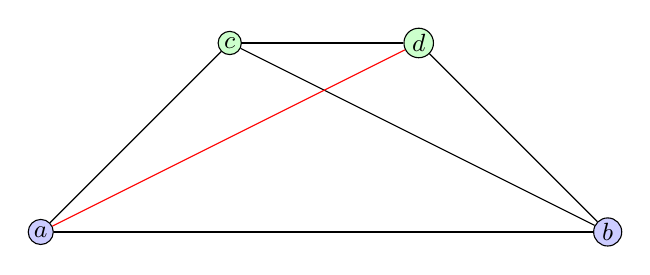
\begin{tikzpicture}[x=1.2cm,y=1.2cm,
    every node/.style={circle,draw,inner sep=1pt,font=\small}]

    % Place K4 vertices
    \node[fill=blue!20]  (a) at (-1,0)   {$a$};
    \node[fill=blue!20]  (b) at (5,0)    {$b$};
    \node[fill=green!20] (c) at (1,2)    {$c$};
    \node[fill=green!20] (d) at (3,2)    {$d$};

    % All edges of K4, with a--d in red
    \foreach \u/\v in {a/b,a/c,b/c,b/d,c/d} {
      \draw (\u) -- (\v);
    }
    \draw[red] (a) -- (d);


    % Track labels

  \end{tikzpicture}
  \caption{Un $K_4$ dibujado con dos ``colores de track''. Ningún orden de $a,b,c,d$ puede evitar crear un triple $x<y<z$ con $\{x,z\}\in E$ donde $y$ comparta track con $x$ o $z$, así que hacen falta al menos tres tracks.}
  \label{fig:K4-tracks}
\end{figure}

\subsection{Una cota de grado: $\Delta(G)\le 2k$}

\begin{lemma}[Cota de grado para diseños en $k$ tracks]
\label{lem:degree-bound}
Sea $G = (V,E)$ un grafo simple no dirigido representable por vecinos más
cercanos en $k$ tracks. Es decir, existe un diseño $(\tau,p)$ con
\[
  \tau : V \to \{1,\dots,k\}, \qquad
  p : V \to \{1,\dots,|V|\}
\]
tal que cada arista es legal:
\[
  \forall \{u,v\}\in E,\quad
  v \in N_{\mathrm{legal}}(u)
  \quad\text{(equivalentemente } u \in N_{\mathrm{legal}}(v)\text{)}.
\]
Entonces para todo vértice $v\in V$ se cumple
\[
  \deg_G(v) \le 2k.
\]
En particular, el grado máximo $\Delta(G)$ satisface
\[
  \Delta(G) \le 2k.
\]
\end{lemma}

\begin{proof}
Fijamos $v\in V$. Para cada track $t$, sea $V_t=\{x:\tau(x)=t\}$ y definimos
$\operatorname{pred}_t(v),\operatorname{succ}_t(v)$ como antes. El conjunto
de vecinos legales es
\[
  N_{\mathrm{legal}}(v)
  =
  \{\operatorname{pred}_1(v),\operatorname{succ}_1(v),\dots,
    \operatorname{pred}_k(v),\operatorname{succ}_k(v)\}
  \setminus\{\text{inexistente}\}.
\]
Por representabilidad por vecinos más cercanos,
\[
  N_G(v) \subseteq N_{\mathrm{legal}}(v),
\]
y entonces
\[
  \deg_G(v) = |N_G(v)| \le |N_{\mathrm{legal}}(v)|.
\]

Para cada track $t$, a lo sumo dos vértices pueden aparecer en
$N_{\mathrm{legal}}(v)$ provenientes del track $t$, a saber
$\operatorname{pred}_t(v)$ y $\operatorname{succ}_t(v)$ si existen.
Definimos
\[
  S_t(v) :=
    \{\operatorname{pred}_t(v),\operatorname{succ}_t(v)\}
    \setminus\{\text{inexistente}\},
\]
entonces $|S_t(v)|\le 2$ y
\[
  N_{\mathrm{legal}}(v)
  = \bigcup_{t=1}^k S_t(v).
\]
Por lo tanto,
\[
  |N_{\mathrm{legal}}(v)|
  \le \sum_{t=1}^k |S_t(v)|
  \le \sum_{t=1}^k 2
  = 2k.
\]
Así, $\deg_G(v)\le 2k$ para todo $v$, y tomando el máximo se obtiene
$\Delta(G)\le 2k$.
\end{proof}

\begin{corollary}[Cota inferior de tracks basada en el grado]
\label{cor:tracks-from-degree}
Si $G$ es representable por vecinos más cercanos en $k$ tracks, entonces
\[
  k \;\ge\; \Bigl\lceil\frac{\Delta(G)}{2}\Bigr\rceil.
\]
\end{corollary}
La Figura~\ref{fig:delta5-example} muestra un vértice de grado~5, lo que
fuerza al menos tres tracks por el Corolario~\ref{cor:tracks-from-degree}.
\begin{figure}[ht]
  \centering
  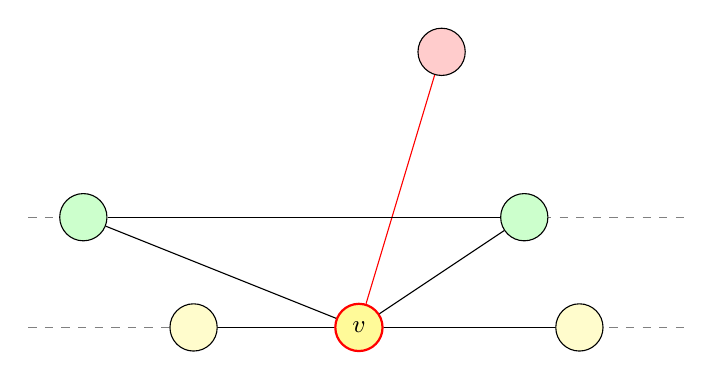
\begin{tikzpicture}[x=1.4cm,y=1.4cm,
    every node/.style={circle,draw,inner sep=1pt,minimum size=6mm,font=\small}]

    % Dashed horizontal lines
    \draw[dashed,gray] (-3,0) -- (3,0);
    \draw[dashed,gray] (-3,1) -- (3,1);

    % Central vertex v
    \node[fill=yellow!40,draw=red,thick] (v) at (0,0) {$v$};

    % Five neighbors around
    \node[fill=yellow!20]  (n1) at (2,0)   {};
    \node[fill=green!20]  (n2) at (1.5,1.0) {};
    \node[fill=red!20]   (n3) at (0.75,2.5)   {};
    \node[fill=green!20] (n4) at (-2.5,1.0) {};
    \node[fill=yellow!20] (n5) at (-1.5,0)  {};

    % Edges: v--n3 in red, others black
    \foreach \w in {n1,n2,n4,n5} {
      \draw (v) -- (\w);
    }
    \draw[red] (v) -- (n3);
    \draw[black] (n2) -- (n4);

  \end{tikzpicture}
  \caption{Un vértice de grado $5$: por $\Delta(G)\le 2k$, esto implica $k\ge 3$.}
  \label{fig:delta5-example}
\end{figure}

\begin{proof}
Sale directamente del Lema~\ref{lem:degree-bound}.
\end{proof}



\begin{figure}[ht]
  \centering
  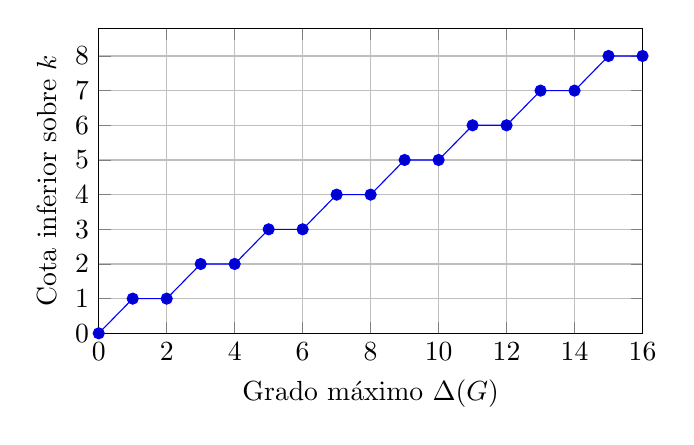
\begin{tikzpicture}
    \begin{axis}[
      width=0.7\textwidth,
      height=0.45\textwidth,
      xlabel={Grado máximo $\Delta(G)$},
      ylabel={Cota inferior sobre $k$},
      ymin=0,
      xmin=0,
      xmax=16,
      xtick={0,2,4,6,8,10,12,14,16},
      ytick={0,1,2,3,4,5,6,7,8},
      grid=both,
    ]
      % Stepwise plot of k ≥ ceil(Δ/2)
      \addplot+[mark=*] coordinates {
        (0,0)
        (1,1)
        (2,1)
        (3,2)
        (4,2)
        (5,3)
        (6,3)
        (7,4)
        (8,4)
        (9,5)
        (10,5)
        (11,6)
        (12,6)
        (13,7)
        (14,7)
        (15,8)
        (16,8)
      };
    \end{axis}
  \end{tikzpicture}
  \caption{Cota inferior sobre el número de tracks:
    $k \ge \lceil \Delta(G)/2\rceil$. En particular, $\Delta(G)\ge 5$
    fuerza $k\ge 3$.}
\end{figure}


\subsection{Cota de aristas para dos tracks: a lo sumo \texorpdfstring{$2n-3$}{2n-3}}

Hasta ahora vimos que un diseño en $k$ tracks para vecinos más cercanos
fuerza $\Delta(G)\le 2k$ (Lema~\ref{lem:degree-bound}). Para $k=2$ podemos
decir mucho más: no sólo el grado máximo es a lo sumo $4$, sino que el
\emph{número total de aristas} es a lo sumo $2n-3$ para un grafo de $n$
vértices. Esto coincide con la cota extremal conocida para grafos
outerplanos.

Trabajamos respecto de un diseño fijo en $2$ tracks $(\tau,p)$ y su grafo
anfitrión $H(\tau,p)$.

\begin{definition}[Grado hacia la izquierda]
Dado un orden lineal $v_1,\dots,v_n$ de $V(G)$ inducido por $p$, el
\emph{grado hacia la izquierda} de $v_i$ se define como
\[
  \deg^-(v_i)
  := \bigl|\{\,u\in N_G(v_i) : p(u) < p(v_i)\,\}\bigr|.
\]
Equivalentemente, $\deg^-(v_i)$ cuenta los vecinos de $v_i$ estrictamente
a su izquierda en el orden global.
\end{definition}

Cada arista $\{u,v\}$ se cuenta exactamente una vez en la suma de grados
hacia la izquierda, en su extremo derecho.

\begin{lemma}[A lo sumo un predecesor por track]
\label{lem:left-degree-two}
Sea $G$ representable por vecinos más cercanos en $k$ tracks respecto de
$(\tau,p)$, y sea $v\in V(G)$. Entonces para cada track
$t\in\{1,\dots,k\}$, $v$ tiene a lo sumo un vecino en el track $t$ a su
izquierda. En particular,
\[
  \deg^-(v) \;\le\; k
\]
para todo vértice $v$.
\end{lemma}

\begin{proof}
Fijamos $v$ y un track $t$. Por definición, el único candidato a vecino a la
izquierda de $v$ en el track $t$ que puede ser legal en el grafo anfitrión
es $\operatorname{pred}_t(v)$ (si existe). No pueden existir dos vecinos
distintos $x,y$ en el track $t$ con $p(x)<p(y)<p(v)$ y ambos adyacentes a
$v$, porque sólo el más cercano a la izquierda puede ser un predecesor
legal en ese track.

Por lo tanto, en cada track $t$ hay a lo sumo un vecino de $v$ a la izquierda.
Sumando sobre los $k$ tracks obtenemos $\deg^-(v)\le k$.
\end{proof}

\begin{theorem}[Cota de aristas para diseños en dos tracks]
\label{thm:edge-bound-2tracks}
Sea $G$ un grafo simple finito de $n$ vértices representable por vecinos más
cercanos en $2$ tracks. Entonces
\[
  |E(G)| \;\le\; 2n - 3.
\]
Además, para todo $n\ge 2$ existe un grafo de este tipo con exactamente
$2n-3$ aristas.
\end{theorem}

\begin{proof}
Sea $(\tau,p)$ un diseño en $2$ tracks y sea $H=H(\tau,p)$ su grafo
anfitrión. Como $G$ es subgrafo de $H$, alcanza con demostrar
$|E(H)|\le 2n-3$.

Escribimos $V=\{v_1,\dots,v_n\}$ en orden creciente de $p$, de forma que
$p(v_i)=i$. Cada arista de $H$ tiene un único extremo derecho, entonces
\[
  |E(H)| = \sum_{i=1}^n \deg_H^-(v_i).
\]

Ahora:
\begin{itemize}[leftmargin=2em]
  \item Para $v_1$, no hay vértices a la izquierda, entonces
        $\deg_H^-(v_1)=0$.
  \item Para $v_2$, el único vértice a la izquierda es $v_1$, así que
        $\deg_H^-(v_2)\le 1$ en cualquier grafo simple.
  \item Para cada $i\ge 3$, el Lema~\ref{lem:left-degree-two} con $k=2$
        da $\deg_H^-(v_i)\le 2$.
\end{itemize}
Por lo tanto,
\[
  |E(H)|
  = \sum_{i=1}^n \deg_H^-(v_i)
  \;\le\; 0 + 1 + 2(n-2)
  = 2n - 3.
\]
Como $G$ es subgrafo de $H$, también vale $|E(G)|\le |E(H)|\le 2n-3$.

\medskip
Para ver que la cota es ajustada, fijemos $n\ge 2$ y construyamos un diseño
en $2$ tracks sobre los vértices $v_1,\dots,v_{n-1},w$ como sigue:
\begin{itemize}[leftmargin=2em]
  \item Ponemos $v_1,\dots,v_{n-1}$ en el track~1 en el orden
        $p(v_i)=i$ y conectamos todos los pares consecutivos
        $\{v_i,v_{i+1}\}$, formando un camino de longitud $n-2$.
  \item Ponemos $w$ en el track~2 a la extrema derecha, $p(w)=n$.
\end{itemize}
En el track~1 tenemos $n-2$ aristas. Para los vecinos de track cruzado:
\begin{itemize}[leftmargin=2em]
  \item Para cada $v_i$, $w$ es el vértice más cercano en el track~2
        a la derecha, luego $\{v_i,w\}$ es una arista cruzada legal.
  \item Hay $n-1$ vértices $v_i$ de este tipo.
\end{itemize}
Así, $H$ tiene $(n-2)$ aristas en el track~1 y $(n-1)$ aristas cruzadas
a $w$, sumando en total
\[
  (n-2) + (n-1) = 2n - 3
\]
aristas. Tomando $G=H$ vemos que la cota es ajustada para todo $n\ge 2$.
\end{proof}

La Figura~\ref{fig:two-track-extremal} muestra la construcción extremal para
$n=6$, y la Figura~\ref{fig:two-track-extremal-growth} muestra cómo cada
vértice nuevo puede aportar a lo sumo dos aristas nuevas cuando construimos
un grafo de este tipo de izquierda a derecha en el orden global.

\begin{figure}[ht]
  \centering
  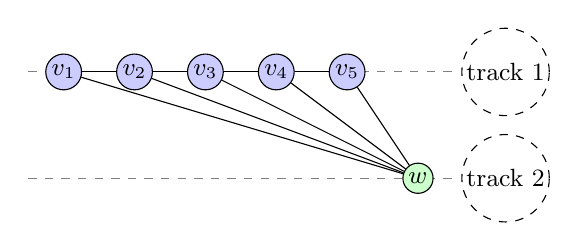
\begin{tikzpicture}[scale=0.9,
    every node/.style={circle,draw,inner sep=1.1pt,font=\small}]
    % Track y-coordinates
    \def\yone{1.5}
    \def\ytwo{0.0}

    % Tracks
    \draw[dashed,gray] (0.5,\yone) -- (6.5,\yone)
      node[right=1mm,black] {$\text{track }1$};
    \draw[dashed,gray] (0.5,\ytwo) -- (6.5,\ytwo)
      node[right=1mm,black] {$\text{track }2$};

    % Vertices on track 1: v1,...,v5
    \foreach \i in {1,...,5} {
      \node[fill=blue!20] (v\i) at (\i,\yone) {$v_{\i}$};
    }

    % Vertex w on track 2 at the far right
    \node[fill=green!20] (w) at (6,\ytwo) {$w$};

    % Path edges on track 1
    \foreach \i/\j in {1/2,2/3,3/4,4/5} {
      \draw (v\i) -- (v\j);
    }

    % Cross edges from w to all v_i
    \foreach \i in {1,...,5} {
      \draw (w) -- (v\i);
    }

  \end{tikzpicture}
  \caption{Un grafo anfitrión extremal en $2$ tracks con $n=6$ vértices:
  un camino $v_1-\dots-v_5$ en el track~1 y un único vértice $w$ en el
  track~2, unido a todos los $v_i$. Esto tiene $(6-2)+(6-1)=9=2n-3$ aristas.}
  \label{fig:two-track-extremal}
\end{figure}

\begin{figure}[ht]
  \centering
  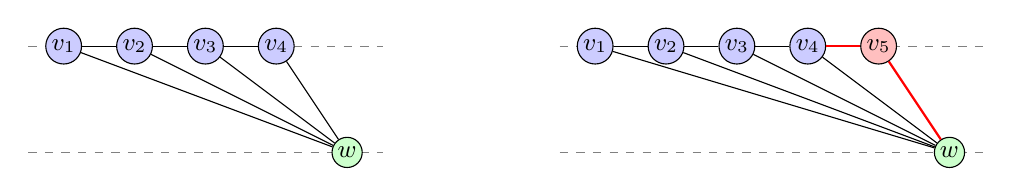
\begin{tikzpicture}[scale=0.9,
    every node/.style={circle,draw,inner sep=1.1pt,font=\small}]

    %==================== Before: n-1 vertices ====================
    \begin{scope}
      \def\yone{1.5}
      \def\ytwo{0.0}

      % Tracks
      \draw[dashed,gray] (0.5,\yone) -- (5.5,\yone);
      \draw[dashed,gray] (0.5,\ytwo) -- (5.5,\ytwo);

      % Vertices on track 1: v1,...,v4
      \foreach \i in {1,...,4} {
        \node[fill=blue!20] (a\i) at (\i,\yone) {$v_{\i}$};
      }

      % Vertex w on track 2
      \node[fill=green!20] (aw) at (5,\ytwo) {$w$};

      % Path edges on track 1
      \foreach \i/\j in {1/2,2/3,3/4} {
        \draw (a\i) -- (a\j);
      }

      % Cross edges from w to all v_i
      \foreach \i in {1,...,4} {
        \draw (aw) -- (a\i);
      }

    \end{scope}

    %==================== After: n vertices ====================
    \begin{scope}[xshift=7.5cm]
      \def\yone{1.5}
      \def\ytwo{0.0}

      % Tracks
      \draw[dashed,gray] (0.5,\yone) -- (6.5,\yone);
      \draw[dashed,gray] (0.5,\ytwo) -- (6.5,\ytwo);

      % Vertices on track 1: v1,...,v5
      \foreach \i in {1,...,4} {
        \node[fill=blue!20] (b\i) at (\i,\yone) {$v_{\i}$};
      }
      % New vertex v5
      \node[fill=red!25] (b5) at (5,\yone) {$v_{5}$};

      % Vertex w on track 2
      \node[fill=green!20] (bw) at (6,\ytwo) {$w$};

      % Old path edges
      \foreach \i/\j in {1/2,2/3,3/4} {
        \draw (b\i) -- (b\j);
      }

      % New path edge and cross edge in red
      \draw[thick,red] (b4) -- (b5);
      \draw[thick,red] (b5) -- (bw);

      % Old cross edges from w to v1,...,v4
      \foreach \i in {1,...,4} {
        \draw (bw) -- (b\i);
      }

    \end{scope}

  \end{tikzpicture}
  \caption{Vista incremental de la familia extremal. Cuando agregamos un
  vértice nuevo en el extremo derecho del track principal (acá $v_5$),
  podemos conectarlo a lo sumo con dos vecinos nuevos a su izquierda:
  el extremo anterior del camino y el vértice especial $w$ del otro track.
  Esto aporta exactamente dos aristas nuevas, consistente con la cota
  $|E|\le 2n-3$.}
  \label{fig:two-track-extremal-growth}
\end{figure}


\subsection{Dos vértices de bajo grado en los extremos del orden}

La prueba del Teorema~\ref{thm:edge-bound-2tracks} señala naturalmente a los
primeros y últimos vértices en el orden global. Para $k=2$ siempre tienen
grado a lo sumo~$2$.

\begin{lemma}[Extremos con grado a lo sumo dos]
\label{lem:endpoints-degree-two}
Sea $G$ representable por vecinos más cercanos en $2$ tracks con diseño
$(\tau,p)$ sobre los vértices $v_1,\dots,v_n$ en orden creciente de $p$.
Entonces
\[
  \deg_G(v_1) \le 2
  \quad\text{y}\quad
  \deg_G(v_n) \le 2.
\]
\end{lemma}

\begin{proof}
Por definición,
\[
  N_{\mathrm{legal}}(v)
  =
  \{\operatorname{pred}_1(v),\operatorname{succ}_1(v),
    \operatorname{pred}_2(v),\operatorname{succ}_2(v)\}
  \setminus\{\text{inexistente}\}.
\]

Para $v_1$ no hay vértices a la izquierda en ningún track, así que tanto
$\operatorname{pred}_1(v_1)$ como $\operatorname{pred}_2(v_1)$ son inexistentes.
Los únicos vecinos legales posibles de $v_1$ son sus dos sucesores,
$\operatorname{succ}_1(v_1)$ y $\operatorname{succ}_2(v_1)$, a lo sumo uno en
cada track. Entonces $|N_{\mathrm{legal}}(v_1)|\le 2$, y como $G$ es un
subgrafo del grafo anfitrión, $\deg_G(v_1)\le |N_{\mathrm{legal}}(v_1)|\le 2$.

Simétricamente, $v_n$ no tiene vértices a la derecha en ningún track, entonces
$\operatorname{succ}_1(v_n)$ y $\operatorname{succ}_2(v_n)$ son inexistentes,
y sus únicos vecinos legales posibles son los dos predecesores
$\operatorname{pred}_1(v_n)$ y $\operatorname{pred}_2(v_n)$. De nuevo,
$|N_{\mathrm{legal}}(v_n)|\le 2$, luego $\deg_G(v_n)\le 2$.
\end{proof}

En particular, todo grafo conexo representable por vecinos más cercanos en
$2$ tracks tiene al menos dos vértices de grado a lo sumo~$2$, ubicados en
los extremos izquierdo y derecho del orden global. Esto es exactamente lo
que hace falta para arrancar un argumento inductivo de ``pelado'': eliminar
$v_1$ o $v_n$, aplicar la cota de aristas al grafo restante de $(n-1)$
vértices y luego agregar de vuelta un vértice de grado a lo sumo~$2$.

\begin{figure}[ht]
  \centering
  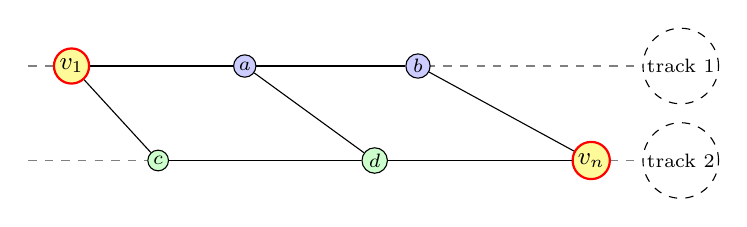
\begin{tikzpicture}[x=1.1cm,y=1.0cm,
    every node/.style={circle,draw,inner sep=1pt,font=\scriptsize}]

    % Tracks
    \draw[dashed,gray] (0.5,1.2) -- (7.5,1.2)
      node[right=1mm,black] {\scriptsize track 1};
    \draw[dashed,gray] (0.5,0.0) -- (7.5,0.0)
      node[right=1mm,black] {\scriptsize track 2};

    % Endpoints
    \node[fill=yellow!40,draw=red,thick,font=\small] (v1) at (1,1.2) {$v_1$};
    \node[fill=yellow!40,draw=red,thick,font=\small] (vn) at (7,0.0) {$v_n$};

    % Middle vertices
    \node[fill=blue!20] (a)  at (3,1.2) {$a$};
    \node[fill=blue!20] (b)  at (5,1.2) {$b$};
    \node[fill=green!20] (c) at (2,0.0) {$c$};
    \node[fill=green!20] (d) at (4.5,0.0) {$d$};

    % Possible neighbors of v1: one on each track
    \draw (v1) -- (a);
    \draw (v1) -- (c);

    % Possible neighbors of vn: one on each track
    \draw (vn) -- (b);
    \draw (vn) -- (d);

    % Some extra edges among middle vertices (just for context)
    \draw (a) -- (b);
    \draw (c) -- (d);
    \draw (a) -- (d);

  \end{tikzpicture}
  \caption{En un diseño de vecinos más cercanos en $2$ tracks, el primer
  vértice $v_1$ sólo puede ver un sucesor en cada track, y el último vértice
  $v_n$ sólo puede ver un predecesor en cada track. Por eso ambos tienen
  grado a lo sumo~$2$.}
  \label{fig:endpoints-degree-two}
\end{figure}


% =====================================================
\section{Ejemplos: ciclos y caminos con una arista extra}
% =====================================================

Ahora miramos familias concretas de grafos y determinamos sus números de
tracks, respondiendo más en concreto cuándo alcanza con $k=1$ versus cuándo
hace falta $k=2$.

\subsection{Ciclos: $C_n$ necesita exactamente dos tracks}

\begin{theorem}[Número de tracks de un ciclo]
\label{thm:cycle}
Para todo entero $n \ge 3$, el ciclo $C_n$ es representable por vecinos más
cercanos en $k=2$ tracks, pero no en $k=1$. En particular,
\[
  \operatorname{tn}(C_n) = 2.
\]
\end{theorem}

\begin{proof}
\emph{Paso 1: $C_n$ no es representable con $k=1$.}

Supongamos, para llegar a una contradicción, que $C_n$ es representable
por vecinos más cercanos en $1$ track. Entonces existe un diseño
$(\tau,p)$ en $1$ track tal que todas las aristas de $C_n$ son legales.

Como $k=1$, todos los vértices están en el track $1$, y podemos escribir
el orden lineal como
\[
  v_1, v_2, \dots, v_n, \quad \text{donde } p(v_i) = i.
\]
En el único track, las únicas aristas legales posibles son entre
vértices consecutivos:
\[
  E\bigl(H(\tau,p)\bigr) \subseteq \{\{v_i,v_{i+1}\} : 1\le i\le n-1\},
\]
así que $H(\tau,p)$ es un bosque (de hecho, un camino) y no contiene ciclos.
Pero $C_n$ es un ciclo, así que no puede ser subgrafo de $H(\tau,p)$,
contradiciendo la representabilidad por vecinos más cercanos.

Luego $C_n$ no es representable con $k=1$.

\medskip
\noindent\emph{Paso 2: diseño explícito en $2$ tracks para $C_n$.}

Etiquetamos los vértices de $C_n$ como $v_1,\dots,v_n$ con aristas
\[
  E(C_n) = \bigl\{\{v_i,v_{i+1}\} : 1\le i \le n-1\bigr\} \cup \{\{v_n,v_1\}\}.
\]

\smallskip
\noindent\emph{Orden global.}
Tomamos $p(v_i)=i$ para todo $i$.

\smallskip
\noindent\emph{Asignación de tracks.}
Usamos dos tracks $\{1,2\}$ y definimos
\[
  \tau(v_1) = \tau(v_n) = 1, \qquad
  \tau(v_i) = 2 \quad \text{para } 2 \le i \le n-1.
\]
Así, el track $1$ tiene los vértices $\{v_1,v_n\}$ y el track $2$
tiene $\{v_2,\dots,v_{n-1}\}$.

Chequeamos ahora que cada arista de $C_n$ es legal.

\smallskip
\noindent\emph{Aristas interiores en el track 2.}
Para $2\le i\le n-2$, tanto $v_i$ como $v_{i+1}$ están en el track $2$ y son
consecutivos allí, entonces
\[
  \operatorname{succ}_2(v_i) = v_{i+1},\quad
  \operatorname{pred}_2(v_{i+1}) = v_i.
\]
Por lo tanto cada $\{v_i,v_{i+1}\}$ con $2\le i\le n-2$ es legal.

\smallskip
\noindent\emph{Aristas $\{v_1,v_2\}$ y $\{v_{n-1},v_n\}$.}
Estas involucran un vértice del track $1$ y otro del track $2$.
Chequeando los vecinos más cercanos en el track opuesto vemos que:
\begin{itemize}[leftmargin=2em]
  \item $v_2$ es el vértice más cercano del track~2 a la derecha de $v_1$,
        y $v_1$ es el vértice más cercano del track~1 a la izquierda de $v_2$,
        así que $\{v_1,v_2\}$ es legal.
  \item $v_n$ es el vértice más cercano del track~1 a la derecha de
        $v_{n-1}$ y $v_{n-1}$ es el más cercano del track~2 a la izquierda
        de $v_n$, así que $\{v_{n-1},v_n\}$ es legal.
\end{itemize}

\smallskip
\noindent\emph{Arista $\{v_n,v_1\}$.}
Ambos extremos están en el track $1$ y son los únicos vértices de ese track,
entonces
\[
  \operatorname{succ}_1(v_1) = v_n,\quad
  \operatorname{pred}_1(v_n) = v_1,
\]
y $\{v_n,v_1\}$ es legal.

\smallskip
Por lo tanto $(\tau,p)$ es un diseño en $2$ tracks en el que todas las
aristas de $C_n$ son legales, así que $C_n$ es representable por vecinos
más cercanos en $2$ tracks.

Combinado con la no representabilidad para $k=1$, obtenemos
$\operatorname{tn}(C_n)=2$.
\end{proof}

\begin{figure}[h]
  \centering
  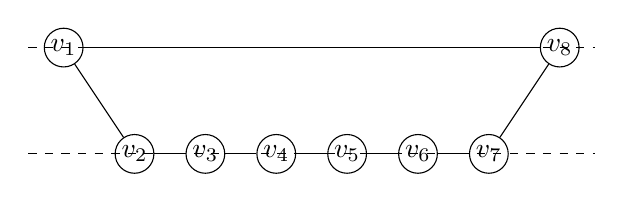
\begin{tikzpicture}[scale=0.9, every node/.style={circle,draw,inner sep=1.1pt}]
    % Track y-coordinates
    \def\yone{1.5}
    \def\ytwo{0}

    % Vertices v1,...,v8 on x=1,...,8
    \foreach \i in {1,...,8} {
      \pgfmathsetmacro{\x}{\i}
      % Track assignment: v1,v8 on track 1; others on track 2
      \ifnum\i=1
        \node (v\i) at (\x,\yone) {$v_{\i}$};
      \else\ifnum\i=8
        \node (v\i) at (\x,\yone) {$v_{\i}$};
      \else
        \node (v\i) at (\x,\ytwo) {$v_{\i}$};
      \fi\fi
    }

    % Draw tracks as dashed lines
    \draw[dashed] (0.5,\yone) -- (8.5,\yone);
    \draw[dashed] (0.5,\ytwo) -- (8.5,\ytwo);

    % Cycle edges: (v1-v2-...-v8-v1)
    \foreach \i/\j in {1/2,2/3,3/4,4/5,5/6,6/7,7/8,8/1} {
      \draw (v\i) -- (v\j);
    }
  \end{tikzpicture}
  \caption{Un diseño en $2$ tracks de $C_8$ con $v_1,v_8$ en el track~1 y $v_2,\dots,v_7$ en el track~2.}
\end{figure}

\subsection{Un camino más una arista extra}

Mostramos ahora que un camino con una sola arista adicional siempre es
representable en $2$ tracks. Es un ejemplo simple de grafo que ya
\emph{no} es un bosque lineal pero igual necesita sólo $k=2$ tracks.

\begin{theorem}[Caminos con una arista extra]
\label{thm:path-plus-edge}
Sea $G$ un grafo conexo simple no dirigido obtenido así:
\begin{itemize}[leftmargin=2em]
  \item $V = \{v_1,\dots,v_n\}$ para algún $n \ge 2$,
  \item $E$ contiene todas las aristas del camino $\{v_i,v_{i+1}\}$ para
        $i = 1,\dots,n-1$,
  \item y además una única arista extra $e^\star = \{v_a,v_b\}$ con
        $1 \le a < b \le n$.
\end{itemize}
Entonces $G$ es representable por vecinos más cercanos en $2$ tracks.
\end{theorem}
La Figura~\ref{fig:path-plus-edge-interior} ilustra la construcción para una
arista extra $\{v_3,v_7\}$. La misma idea funciona cuando uno o ambos
extremos de la arista extra están en los extremos del camino. Como un grafo
representable por vecinos más cercanos en $1$ track es un bosque lineal
(Remarca~\ref{rem:what-k1-means}) y nuestros grafos contienen un ciclo, no
pueden ser representables en $1$ track. Junto con la construcción anterior,
esto muestra que su número de tracks de vecinos más cercanos es exactamente $2$.

\begin{figure}[ht]
  \centering
  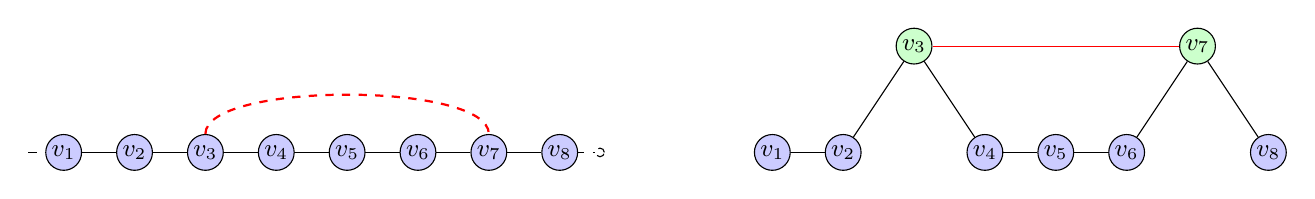
\begin{tikzpicture}[scale=0.9,
    every node/.style={circle,draw,inner sep=1.1pt,font=\small}]

    %==================== Before: 1-track layout ====================
    \begin{scope}
      % Single track
      \def\ybefore{0}
      \draw[dashed] (0.5,\ybefore) -- (8.5,\ybefore)
        node[right] {};

      % Vertices v1,...,v8 on the single track
      \foreach \i in {1,...,8} {
        \node[fill=blue!20] (u\i) at (\i,\ybefore) {$v_{\i}$};
      }

      % Path edges (all legal in 1-track layout)
      \foreach \i/\j in {1/2,2/3,3/4,4/5,5/6,6/7,7/8} {
        \draw (u\i) -- (u\j);
      }

      % Extra edge {v3,v7}: not a nearest-neighbor edge here
      \draw[thick,red,dashed] (u3) .. controls +(0,1.0) and +(0,1.0) .. (u7);


    \end{scope}

    %==================== After: 2-track layout ====================
    \begin{scope}[xshift=10cm]
      % Track y-coordinates
      \def\yone{0}
      \def\ytwo{1.5}

      % Vertices v1,...,v8
      \foreach \i in {1,...,8} {
        \ifnum\i=3
          \node[fill=green!20] (v\i) at (\i,\ytwo) {$v_{\i}$}; % a = 3 elevated
        \else\ifnum\i=7
          \node[fill=green!20] (v\i) at (\i,\ytwo) {$v_{\i}$}; % b = 7 elevated
        \else
          \node[fill=blue!20]  (v\i) at (\i,\yone) {$v_{\i}$};
        \fi\fi
      }

      % Path edges (still all legal)
      \foreach \i/\j in {1/2,2/3,3/4,4/5,5/6,6/7,7/8} {
        \draw (v\i) -- (v\j);
      }

      \draw[red] (v3) -- (v7);
      % Caption under the right subgraph
    \end{scope}

  \end{tikzpicture}
  \caption{Un camino $v_1-\cdots-v_8$ con una arista extra $\{v_3,v_7\}$. 
  Izquierda: el diseño natural en $1$ track del camino; la arista extra
  (roja, punteada) salta varios vértices y no es una arista de vecinos más
  cercanos. 
  Derecha: moviendo $v_3$ y $v_7$ al track~2, obtenemos un diseño en $2$
  tracks en el que la arista extra (roja sólida) pasa a ser legal mientras
  que todas las aristas del camino siguen siendo legales.}
  \label{fig:path-plus-edge-interior}
\end{figure}


\begin{proof}
Mantenemos el orden natural $p(v_i)=i$ y sólo modificamos la asignación de
tracks.

\smallskip
\noindent\emph{Paso 1: arrancamos del camino.}
Para el camino puro $P_n$ con aristas $\{v_i,v_{i+1}\}$, el diseño
\[
  \tau^{(1)}(v_i) = 1\quad\text{para todo }i,
  \qquad p(v_i)=i,
\]
es un diseño de vecinos más cercanos en $1$ track: cada arista
$\{v_i,v_{i+1}\}$ conecta vértices consecutivos en el track $1$.

\smallskip
\noindent\emph{Paso 2: movemos los extremos de la arista extra al track 2.}
Ahora agregamos la arista extra $e^\star=\{v_a,v_b\}$ con $a<b$, mantenemos
el mismo orden global $p$ y definimos una nueva asignación de tracks $\tau$
por
\[
  \tau(v_i) =
  \begin{cases}
    2, & \text{si } i \in \{a,b\},\\[2pt]
    1, & \text{en otro caso}.
  \end{cases}
\]
Así, sólo $v_a$ y $v_b$ están en el track $2$; todos los demás vértices
están en el track $1$.

Chequeamos que todas las aristas de $G$ son legales bajo $(\tau,p)$.

\smallskip
\noindent\emph{Paso 3: aristas del camino no incidentes en $v_a$ o $v_b$.}
Si $i\notin\{a-1,a,b-1,b\}$, entonces $\{v_i,v_{i+1}\}$ no es incidente
ni en $v_a$ ni en $v_b$ y ambos extremos están en el track $1$. Son
consecutivos en el orden global y no hay otro vértice del track~1 entre ellos;
por lo tanto
\[
  \operatorname{succ}_1(v_i)=v_{i+1},\quad
  \operatorname{pred}_1(v_{i+1})=v_i,
\]
y $\{v_i,v_{i+1}\}$ es legal.

\smallskip
\noindent\emph{Paso 4: aristas del camino incidentes en $v_a$ o $v_b$.}
Consideremos las aristas $\{v_{a-1},v_a\}$ y $\{v_a,v_{a+1}\}$ (cuando
esos índices existan). El vecino de $v_a$ inmediatamente a la izquierda en
el track~1 es $v_{a-1}$ y el de la derecha es $v_{a+1}$, entonces
\[
  \operatorname{pred}_1(v_a) = v_{a-1}\text{ (si $a>1$)},\quad
  \operatorname{succ}_1(v_a) = v_{a+1}\text{ (si $a<n$)}.
\]
Así, las aristas $\{v_{a-1},v_a\}$ y $\{v_a,v_{a+1}\}$ son legales.

El mismo argumento aplica a $v_b$: los vértices más cercanos en el track~1 a
la izquierda y a la derecha son $v_{b-1}$ y $v_{b+1}$ (si existen), haciendo
que $\{v_{b-1},v_b\}$ y $\{v_b,v_{b+1}\}$ sean legales.

\smallskip
\noindent\emph{Paso 5: la arista extra $\{v_a,v_b\}$.}
En el track $2$, $v_a$ y $v_b$ son los únicos vértices y $a<b$. Entonces
\[
  \operatorname{succ}_2(v_a) = v_b, \qquad
  \operatorname{pred}_2(v_b) = v_a,
\]
luego $v_b\in N_{\mathrm{legal}}(v_a)$ y $v_a\in N_{\mathrm{legal}}(v_b)$.
Por lo tanto la arista extra es legal.

\smallskip
En conjunto, cada arista de $G$ es legal, así que $G$ es representable por
vecinos más cercanos en $2$ tracks.
\end{proof}

% =====================================================
\section{Planaridad para $k\le 2$}
% =====================================================

Finalmente, mostramos que $k\le 2$ impone restricciones estructurales fuertes:
todo grafo de este tipo es planar.

\begin{theorem}[Planaridad para $k\le 2$]
\label{thm:planarity-k-le-2}
Sea $G$ un grafo simple no dirigido representable por vecinos más cercanos
en $(k)$ tracks con $k\le 2$. Entonces $G$ es planar.
\end{theorem}

\begin{proof}
Tratamos por separado los casos $k=1$ y $k=2$.

\medskip
\noindent\emph{Caso $k=1$.}
Cuando hay un solo track, cada vértice tiene a lo sumo un predecesor y un
sucesor, y toda arista legal conecta vértices consecutivos en el orden del
track. Por lo tanto, cada componente conexa de $G$ es un camino (o un
vértice aislado). Un grafo así es una unión disjunta de caminos y vértices
aislados, luego planar.

\medskip
\noindent\emph{Caso $k=2$: reducción a grafos anfitriones.}
Fijamos un diseño en $2$ tracks $(\tau,p)$ sobre $V$ y sea $H(\tau,p)$ su
grafo anfitrión con todas las aristas legales. Como $G$ es un subgrafo de
$H(\tau,p)$, alcanza con ver que $H(\tau,p)$ es planar.

Ponemos los vértices sobre una recta horizontal en el orden global
$v_1,\dots,v_n$ con $p(v_i)=i$, y escribimos $\tau(v_i)\in\{1,2\}$.
Particionamos las aristas de $H(\tau,p)$ en cuatro clases:

\begin{itemize}[leftmargin=2em]
  \item $E^{(1)}$: aristas entre vértices consecutivos en el track $1$,
  \item $E^{(2)}$: aristas entre vértices consecutivos en el track $2$,
  \item $E_R$: aristas cruzadas donde cada extremo es el vecino más cercano
               en el track opuesto hacia la derecha,
  \item $E_L$: aristas cruzadas donde cada extremo es el vecino más cercano
               en el track opuesto hacia la izquierda.
\end{itemize}

La Figura~\ref{fig:planar-2tracks} ilustra esquemáticamente el dibujo
planar usado en la prueba.
\begin{figure}[ht]
  \centering
  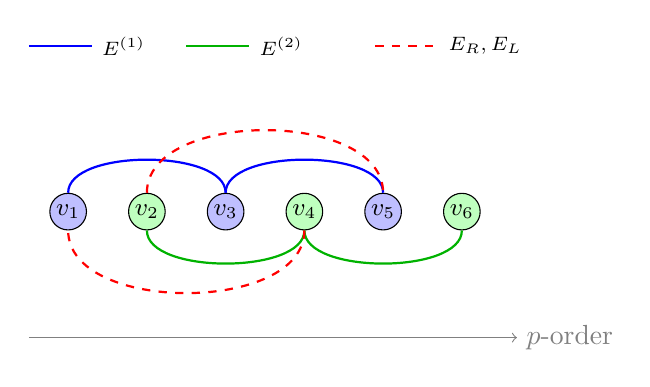
\begin{tikzpicture}[x=1.0cm,y=1cm]

    % Vertices on the x-axis, colored by track
    \foreach \i/\x/\col in {1/1/blue!25,2/2/green!25,3/3/blue!25,4/4/green!25,5/5/blue!25,6/6/green!25} {%
      \node[circle,draw,fill=\col,inner sep=1.2pt,font=\small] (v\i) at (\x,0) {$v_{\i}$};
    }

    % p-order arrow
    \draw[->,gray] (0.5,-1.6) -- (6.7,-1.6) node[right] {$p$-order};

    % Edges on track 1 (E^{(1)}) in upper half-plane
    \draw[thick,blue] (v1) .. controls +(0,0.8) and +(0,0.8) .. (v3);
    \draw[thick,blue] (v3) .. controls +(0,0.8) and +(0,0.8) .. (v5);

    % Edges on track 2 (E^{(2)}) in lower half-plane
    \draw[thick,green!70!black] (v2) .. controls +(0,-0.8) and +(0,-0.8) .. (v4);
    \draw[thick,green!70!black] (v4) .. controls +(0,-0.8) and +(0,-0.8) .. (v6);

    % Cross edges to the right (E_R) in upper half-plane
    \draw[thick,red,dashed] (v2) .. controls +(0,1.3) and +(0,1.3) .. (v5);

    % Cross edges to the left (E_L) in lower half-plane
    \draw[thick,red,dashed] (v4) .. controls +(0,-1.3) and +(0,-1.3) .. (v1);

    % Legend
    \begin{scope}[shift={(0.5,2.1)},font=\scriptsize]
      \draw[blue,thick] (0,0) -- (0.8,0) node[right,black] {$E^{(1)}$};
      \draw[green!70!black,thick] (2.0,0) -- (2.8,0) node[right,black] {$E^{(2)}$};
      \draw[red,thick,dashed] (4.4,0) -- (5.2,0) node[right,black] {$E_R, E_L$};
    \end{scope}

  \end{tikzpicture}
  \caption{Un embedding planar esquemático para un grafo anfitrión en $2$
  tracks: las aristas en el track~1 y las aristas cruzadas hacia la derecha
  se dibujan arriba de la recta, mientras que las aristas en el track~2 y las
  cruzadas hacia la izquierda se dibujan abajo.}
  \label{fig:planar-2tracks}
\end{figure}

Dibujamos:
\begin{itemize}[leftmargin=2em]
  \item todos los vértices $v_1,\dots,v_n$ sobre el eje $x$ en $(i,0)$,
  \item todas las aristas en $E^{(1)}\cup E_R$ como arcos $x$-monótonos en el
        semiplano superior,
  \item todas las aristas en $E^{(2)}\cup E_L$ como arcos $x$-monótonos en el
        semiplano inferior.
\end{itemize}

Es un argumento estándar de órdenes interválicos (omitimos los detalles
de rutina) que:

\begin{itemize}[leftmargin=2em]
  \item las aristas en $E^{(1)}$ forman una familia sin cruces en el
        semiplano superior,
  \item las aristas en $E_R$ forman una familia sin cruces en el semiplano
        superior,
  \item ninguna arista de $E^{(1)}$ se cruza con una arista de $E_R$ en el
        semiplano superior,
  \item por simetría, lo mismo vale para $E^{(2)}$ y $E_L$ en el semiplano
        inferior.
\end{itemize}

Como las aristas dibujadas arriba y abajo sólo se encuentran sobre la recta
horizontal en sus extremos, esto da un embedding planar de $H(\tau,p)$.
Luego $H(\tau,p)$ es planar, y cualquier subgrafo $G$ suyo también lo es.
\end{proof}

Esta restricción de planaridad, junto con las cotas de grado y aristas
probadas antes, se va a aprovechar en la Sección~\ref{sec:recognition} para
diseñar un algoritmo de reconocimiento para diseños de vecinos más cercanos
en $2$ tracks.


% =====================================================
\section{Complejidad: reconocer diseños de vecinos más cercanos en 2 tracks}
% =====================================================


\subsection{El problema de decisión \textsc{2TNN-Layout}}

Fijamos $k=2$ a lo largo de esta sección. Recordemos que un diseño de
vecinos más cercanos en $2$ tracks de un grafo $G=(V,E)$ consiste en:
\begin{itemize}[leftmargin=2em]
  \item una asignación de track $\tau:V\to\{1,2\}$,
  \item y una biyección $p:V\to\{1,\dots,|V|\}$,
\end{itemize}
tal que cada arista $\{u,v\}\in E$ es legal en el sentido de la Sección~1:
cada extremo es el predecesor o sucesor del otro en algún track
(el propio o el opuesto).

\begin{definition}[\textsc{2TNN-Layout}]
\label{def:2tnn-layout-problem}
El problema de decisión \textsc{2TNN-Layout} es:

\medskip\noindent
\emph{Input:} Un grafo simple finito no dirigido $G=(V,E)$.

\smallskip\noindent
\emph{Pregunta:} ¿Existe un diseño ordenado en $2$ tracks $(\tau,p)$ de $G$
tal que $G$ sea representable por vecinos más cercanos en $2$ tracks respecto
de $(\tau,p)$, es decir
\[
  \forall v\in V,\quad N_G(v) \subseteq N_{\mathrm{legal}}(v)?
\]
Equivalentemente, ¿se cumple que $\operatorname{tn}(G)\le 2$ en el sentido
de vecinos más cercanos?
\end{definition}

\subsection{Pertenencia a NP}

\begin{proposition}[\textsc{2TNN-Layout} está en NP]
\label{prop:2tnn-in-NP}
El problema \textsc{2TNN-Layout} pertenece a la clase de complejidad NP.
\end{proposition}

\begin{proof}
Un certificado consiste en un par $(\tau,p)$ con $\tau:V\to\{1,2\}$ y una
biyección $p:V\to\{1,\dots,n\}$. A partir de $(\tau,p)$ podemos computar
todos los predecesores y sucesores a lo largo de cada track en tiempo lineal
y, con eso, los conjuntos de vecinos legales $N_{\mathrm{legal}}(v)$.
Luego verificamos en tiempo $O(|E|)$ que cada arista de $G$ sea legal en
ambos extremos. Por lo tanto \textsc{2TNN-Layout} está en NP.
\end{proof}




% =====================================================
\section{Un algoritmo de reconocimiento para diseños en dos tracks}
% =====================================================
\label{sec:recognition}
Apoyándonos en la mirada de complejidad de la sección anterior, describimos
ahora un procedimiento concreto de decisión para $\operatorname{tn}(G)\le 2$.

Por la Proposición~\ref{prop:tracknumber-components} podemos trabajar
componente conexa por componente, ya que
\(\operatorname{tn}(G) = \max_i \operatorname{tn}(G_i)\).

En toda esta sección, para una componente $H$ escribimos
\[
  n_H := |V(H)|, \qquad m_H := |E(H)|, \qquad \Delta(H) := \max_{v\in V(H)} \deg_H(v).
\]

Nuestro algoritmo tiene dos capas:

\begin{enumerate}[leftmargin=2em]
  \item una \emph{capa de filtros rápidos} con tests estructurales que en
        tiempo $O(n+m)$ o bien certifican \emph{SÍ} o bien \emph{NO} para la
        mayoría de los grafos, y
  \item una \emph{capa de backtracking} sobre los núcleos “difíciles” que
        queden, basada en los cuatro slots de vecinos más cercanos que cada
        vértice puede usar cuando $k=2$.
\end{enumerate}

Organizamos el procedimiento de reconocimiento como una secuencia de
“cortes” estructurales que explicitamente realizan las condiciones necesarias
simples desarrolladas en las secciones previas, seguidos de una búsqueda
exponencial sobre el núcleo restante.


% -----------------------------------------------------
\subsection{Decisiones inmediatas por tamaño y densidad}
% -----------------------------------------------------

Fijamos una componente conexa $H$.

\paragraph{Corte 0: grafos muy chicos.}
Si $n_H \le 3$ entonces $H$ tiene a lo sumo tres aristas y no contiene
un $K_4$, y uno puede escribir fácilmente a mano un diseño de vecinos más
cercanos en $2$ tracks. Tomamos entonces
\[
  n_H \le 3 \quad\Longrightarrow\quad \operatorname{tn}(H) \le 2
\]
como un \emph{SÍ automático}. Esto se chequea en tiempo $O(1)$ por componente.

\paragraph{Corte 1: cota superior de densidad de aristas.}
Por el Teorema~\ref{thm:edge-bound-2tracks}, todo grafo anfitrión en $2$
tracks sobre $n_H$ vértices tiene a lo sumo $2n_H-3$ aristas. Por lo tanto,
cualquier componente con $m_H > 2n_H-3$ no puede tener
$\operatorname{tn}(H)\le 2$.

% -----------------------------------------------------
\subsection{Filtros estructurales lineales}
% -----------------------------------------------------

Una vez que $n_H \ge 4$ y $m_H \le 2n_H-3$, aplicamos tres cortes más,
cada uno justificado por resultados previos.

\paragraph{Corte 2: grado máximo.}
Por el Lema~\ref{lem:degree-bound}, un diseño de vecinos más cercanos en
$k$ tracks satisface $\Delta(H)\le 2k$. Para $k\le 2$ esto implica
\[
  \Delta(H) \le 4.
\]
Así que si alguna vez vemos $\Delta(H)\ge 5$ podemos concluir de inmediato
que $\operatorname{tn}(H)\ge 3$ y devolver \emph{NO}. Computar todos los
grados lleva tiempo $O(n_H + m_H)$.

\paragraph{Corte 3: subgrafo $K_4$.}
El Teorema~\ref{thm:K4-needs-3} muestra que un clique de tamaño $4$ fuerza
al menos tres tracks. Entonces si $H$ contiene un $K_4$ debemos rechazar:
\[
  K_4 \subseteq H \quad\Longrightarrow\quad \operatorname{tn}(H) \ge 3.
\]
Dado que desde el Corte~2 tenemos $\Delta(H)\le 4$, un $K_4$ se puede detectar
en tiempo $O(n_H \Delta(H)^2) = O(n_H)$ intersectando conjuntos de vecinos.

\paragraph{Corte 4: planaridad.}
Por el Teorema~\ref{thm:planarity-k-le-2}, cualquier grafo con
$\operatorname{tn}(H)\le 2$ debe ser planar. Entonces corremos un test de
planaridad en tiempo lineal (por ejemplo Hopcroft--Tarjan) y rechazamos si
$H$ no es planar:
\[
  H \text{ no planar } \quad\Longrightarrow\quad \operatorname{tn}(H)\ge 3.
\]
Esto cuesta $O(n_H + m_H)$.

Luego de los Cortes 1--4, todas las componentes que quedan satisfacen
simultáneamente
\[
  n_H \ge 4,\quad
  m_H \le 2n_H - 3,\quad
  \Delta(H) \le 4,\quad
  H \text{ planar},\quad
  K_4 \not\subseteq H.
\]

% -----------------------------------------------------
\subsection{Casos de SÍ baratos}
% -----------------------------------------------------

Antes de pasar al backtracking, también aprovechamos las construcciones
explícitas de la Sección~5.

\paragraph{Corte 5: bosques lineales.}
Si cada componente de $H$ es un camino o un vértice aislado (un bosque
lineal), entonces $\operatorname{tn}(H)=1$ por lo discutido en la Sección~1,
y respondemos \emph{SÍ}. En el caso conexo esto equivale a testear
\[
  \Delta(H) \le 2\quad \text{y $H$ acíclico}.
\]
La aciclicidad y los grados se pueden chequear en tiempo $O(n_H+m_H)$.

\paragraph{Corte 6: un ciclo con grado máximo $2$.}
La Sección~5 prueba que
\begin{itemize}[leftmargin=2em]
  \item todo ciclo $C_n$ tiene $\operatorname{tn}(C_n)=2$
        (Teorema~\ref{thm:cycle}), y
  \item cualquier grafo obtenido a partir de un camino agregando una arista
        extra también es representable por vecinos más cercanos en $2$ tracks
        (Teorema~\ref{thm:path-plus-edge}).
\end{itemize}
Estos son precisamente los grafos conexos con
\[
  m_H = n_H,\quad \Delta(H) \le 2,
\]
es decir, grafos con tantas aristas como vértices y grado máximo a lo suma
dos.

Así que las componentes conexas con
\[
  m_H = n_H \quad\text{y}\quad \Delta(H)\le 2
\]
son \emph{SÍ automáticos} y nunca llegan a la capa de búsqueda exponencial.
De nuevo, este test es $O(n_H+m_H)$.

(Se puede extender esta familia si uno quiere, usando más teoremas
estructurales, pero lo anterior ya cubre los casos unicíclcos escasos
más comunes.)

% -----------------------------------------------------
\subsection{Reducción a un núcleo planar de grado acotado}
% -----------------------------------------------------
\label{subsec:two-track-core}
Después de los Cortes 0--6, sólo quedan componentes “realmente complicadas”:
grafos planares, libres de $K_4$, con $3 \le \delta(H)\le \Delta(H)\le 4$ y
$m_H\le 2n_H-3$ que no son ni bosques lineales ni ciclos simples ni caminos
con una única arista extra.

En este punto contraemos $H$ a un \emph{núcleo} $H^\star$ más pequeño
eliminando hojas innecesarias y vértices de grado $2$ en caminos, al estilo
de la kernelización estándar.

\begin{itemize}[leftmargin=2em]
  \item Mientras $H$ tenga una hoja $v$ (grado $1$), borramos $v$ y su
        arista incidente. Por el clásico argumento de “volver a pegar la
        hoja”, esto no cambia si existe o no un diseño de vecinos más
        cercanos en $2$ tracks.
  \item Mientras $H$ tenga un vértice de grado $2$ cuyo par de vecinos
        $x,y$ no están adyacentes, contraemos el camino $x-v-y$ en una
        única arista $xy$. Esto preserva la existencia de un diseño: en
        cualquier diseño del grafo contraído, $v$ se puede reinsertar en
        el mismo track entre $x$ e $y$.
\end{itemize}

Llamamos $H^\star$ al resultado, el \emph{núcleo en dos tracks} de $H$.
Es planar, libre de $K_4$, tiene $3 \le \delta(H^\star) \le \Delta(H^\star)
\le 4$, y se puede computar en tiempo $O(n_H+m_H)$.

Si $H^\star$ está vacío, o es un único vértice, o es un único ciclo,
ya sabemos cómo diseñar $H$ a partir de los cortes previos; si no,
$H^\star$ es la instancia sobre la que corremos la búsqueda exponencial.

% -----------------------------------------------------
\subsection{La capa de backtracking}
% -----------------------------------------------------

Sobre $H^\star$ corremos ahora un algoritmo de backtracking exacto pero
exponencial en el tamaño de $H^\star$. La observación clave es que para
$k=2$ cada vértice $v$ puede usar a lo sumo cuatro posiciones legales
de vecinos más cercanos:

\[
  \{\text{pred en el track 1},\ \text{succ en el track 1},\
    \text{pred en el track 2},\ \text{succ en el track 2}\}.
\]

Codificamos estas posiciones como cuatro \emph{slots} abstractos
\[
  \mathsf{1L},\ \mathsf{1R},\ \mathsf{2L},\ \mathsf{2R},
\]
y buscamos asignaciones de aristas incidentes a slots, sujetas a:

\begin{itemize}[leftmargin=2em]
  \item en cada vértice, a lo sumo una arista usa cada slot (cota de grado),
  \item en cada arista $\{u,v\}$, el par de slots elegidos en $u$ y $v$ debe
        ser uno de los ocho pares compatibles que vienen de una relación
        predecesor/sucesor real (en el mismo track o cruzado),
  \item las restricciones inducidas de “estar a la izquierda de” entre
        vértices deben quedar acíclicas, para que se puedan realizar por
        algún orden global $p$.
\end{itemize}

Mantenemos asignaciones parciales de slots y sus implicancias como un CSP
de dominios finitos, y ramificamos en el vértice con menos slots disponibles.
Como $\deg(v)\le 4$ y hay cuatro slots, el factor de ramificación local es
a lo sumo $4! = 24$, y normalmente mucho menor una vez que propagamos las
restricciones.

Una asignación completa y consistente de slots produce un diseño de vecinos
más cercanos en $2$ tracks de $H^\star$ (y por lo tanto de $H$), mientras que
el fracaso en todas las ramas prueba que no existe tal diseño. El argumento
de corrección es estándar y sigue el mismo patrón que otros CSPs de diseño
y orden; omitimos los detalles para no alargar aún más.

En el peor caso esta capa de backtracking corre en tiempo
\[
  O\bigl(c^{n^\star}\bigr),
\]
para alguna constante $c<24$ y $n^\star = |V(H^\star)|$, multiplicado por un
factor polinomial correspondiente a la propagación de restricciones. Este
comportamiento exponencial es esperable: ya el problema estándar de
reconocer el track-number para $k=2$ fijo es NP-completo
(ver Dujmovi\'c et al.~\cite{dujmovic-track-layouts,dujmovic-layered-track}).

% -----------------------------------------------------
\subsection{Algoritmo final y complejidad global}
% -----------------------------------------------------

Podemos resumir ahora todo el procedimiento.

\begin{quote}
\textbf{Algoritmo \textsc{TwoTrackNN}$(G)$}

\emph{Input:} grafo simple finito $G=(V,E)$. \\
\emph{Output:} $1$ si $G$ tiene un diseño de vecinos más cercanos con a lo
sumo dos tracks, $0$ en otro caso.

\begin{enumerate}[leftmargin=2em]
  \item Computar las componentes conexas $G_1,\dots,G_r$ de $G$ \hfill
        (tiempo $O(|V|+|E|)$).
  \item Para cada componente $G_i$:
    \begin{enumerate}[label=(\alph*),leftmargin=1.5em]
      \item Sea $n_i = |V(G_i)|$, $m_i = |E(G_i)|$.
            Si $n_i \le 3$, marcar $G_i$ como \emph{SÍ} y seguir.
      \item Si $m_i > 2n_i - 3$, devolver $0$ (Corte~1).
      \item Computar los grados.  Si $\Delta(G_i) \ge 5$, devolver $0$ (Corte~2).
      \item Testear si hay un $K_4$; si aparece, devolver $0$ (Corte~3).
      \item Correr un test de planaridad en tiempo lineal; si $G_i$ no es
            planar, devolver $0$ (Corte~4).
      \item Si $G_i$ es un bosque lineal, o un ciclo, o un camino con una
            arista extra (Cortes 5 y 6), marcarlo como \emph{SÍ} y seguir.
      \item En otro caso, computar su núcleo $G_i^\star$ borrando hojas y
            suprimiendo vértices de grado $2$ en caminos
            (Sección~\ref{subsec:two-track-core}).
      \item Correr la búsqueda de backtracking basada en slots sobre $G_i^\star$.
            Si falla, devolver $0$; si tiene éxito, marcar $G_i$ como
            \emph{SÍ}.
    \end{enumerate}
  \item Si todas las componentes están marcadas como \emph{SÍ}, devolver $1$.
\end{enumerate}
\end{quote}

Los pasos (1)--(2f) y la reducción al núcleo (2g) en conjunto toman
\[
  O(|V| + |E|)
\]
tiempo.


% =====================================================
\begin{thebibliography}{9}
% =====================================================

\bibitem{dujmovic-track-layouts}
V.~Dujmovi\'c, P.~Morin, and D.~R.~Wood.
Track layouts of graphs.
\emph{Discrete Mathematics \& Theoretical Computer Science} 6(2):497--522, 2004.

\bibitem{dujmovic-layered-track}
V.~Dujmovi\'c and D.~R.~Wood.
Track layouts, layered path decompositions, and leveled planarity.
\emph{Journal of Graph Theory}, to appear.
Preprint available as arXiv:1506.09145.

\bibitem{hopcroft-tarjan}
J.~Hopcroft and R.~Tarjan.
Efficient planarity testing.
\emph{Journal of the ACM} 21(4):549--568, 1974.

\bibitem{queue-number-survey}
D.~Eppstein.
Queue number.
Available at \url{https://en.wikipedia.org/wiki/Queue_number}.

% =====================================================
\end{thebibliography}
% =====================================================
\appendix
% =====================================================
\section{Intentos fallidos de cortes basados en BFS}
% =====================================================
\label{app:failed-bfs-cuts}

Durante el diseño del algoritmo de reconocimiento en
la Sección~\ref{sec:recognition} es tentador buscar condiciones necesarias
extra y ``baratas'' que vengan del comportamiento de un BFS (búsqueda en
anchura). En este apéndice registramos dos ideas de ese estilo que
terminaron siendo inviables: una es demasiado débil como para descartar
algo más allá de la cota de grado, y la otra directamente es falsa (incluso
para grafos muy chicos representables en $2$ tracks).

% -----------------------------------------------------
\subsection{Una cota demasiado débil: a lo sumo tres vértices nuevos por expansión}
% -----------------------------------------------------

Una primera intuición era que, en un diseño de vecinos más cercanos en
$2$ tracks, una expansión de BFS nunca debería descubrir más de dos
vértices nuevos a la vez. Eso es falso en general (un vértice puede tener
grado $4$), pero incluso la versión corregida
\[
  \text{``toda expansión de BFS descubre a lo sumo tres vértices nuevos''}
\]
resulta demasiado débil para ser un corte útil.

De hecho, esta cota viene automáticamente de la restricción local de
grado $\Delta(G)\le 4$ (Lema~\ref{lem:degree-bound}). Si enraizamos un BFS
en algún vértice $r$ y expandimos los vértices uno por uno, para cualquier
vértice $v\neq r$:
\begin{itemize}[leftmargin=2em]
  \item una arista incidente va al padre de $v$ en el BFS y no se cuenta
        como “nueva”,
  \item las restantes a lo sumo $\deg(v)-1\le 3$ aristas incidentes pueden
        llevar a vértices nuevos.
\end{itemize}
Así, la propiedad de “$\le 3$ vértices nuevos por expansión” vale en
todo grafo representable por vecinos más cercanos en $2$ tracks y no agrega
información más allá de la cota de grado; no puede filtrar instancias
adicionales.

% -----------------------------------------------------
\subsection{Una condición falsa de patrones: $2$ nuevos y después $3$ nuevos}
% -----------------------------------------------------

Una idea más ambiciosa fue explotar la \emph{secuencia} de tamaños de capas
del BFS. Sea $L_0,L_1,L_2,\dots$ las capas de un BFS a partir de alguna raíz
elegida, donde $L_i$ es el conjunto de vértices a distancia $i$ de la raíz
y $|L_i|$ es el número de vértices que se descubren \emph{por primera vez}
en esa capa.

La condición tentativa era, informalmente:

\medskip
\begin{quote}
  \emph{En un grafo representable por vecinos más cercanos en $2$ tracks no
  debería existir un BFS en el que una capa con $3$ vértices nuevos esté
  inmediatamente precedida por una capa con $2$ vértices nuevos.}
\end{quote}
\medskip

La idea era usar esto como condición necesaria: si \emph{algún} BFS desde
\emph{alguna} raíz exhibe el patrón
\[
  |L_i| = 2, \quad |L_{i+1}| = 3,
\]
entonces el grafo se descartaría como candidato a tener un diseño en
$2$ tracks de vecinos más cercanos. Sin embargo, el siguiente ejemplo
minúsculo muestra que este patrón sí aparece en un grafo perfectamente
válido de ese tipo.

\begin{figure}[ht]
  \centering
  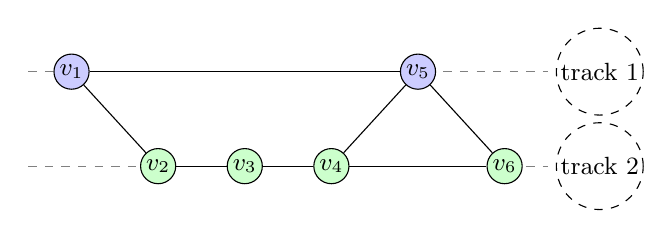
\begin{tikzpicture}[x=1.1cm,y=1.2cm,
    every node/.style={circle,draw,inner sep=1pt,font=\small}]

    % Track lines
    \draw[dashed,gray] (0.5,1.0) -- (6.5,1.0)
      node[right=1mm,black] {$\text{track }1$};
    \draw[dashed,gray] (0.5,0.0) -- (6.5,0.0)
      node[right=1mm,black] {$\text{track }2$};

    % Vertices on track 1
    \node[fill=blue!20]  (v1) at (1,1.0) {$v_1$};
    \node[fill=blue!20]  (v5) at (5,1.0) {$v_5$};

    % Vertices on track 2
    \node[fill=green!20] (v2) at (2,0.0) {$v_2$};
    \node[fill=green!20] (v3) at (3,0.0) {$v_3$};
    \node[fill=green!20] (v4) at (4,0.0) {$v_4$};
    \node[fill=green!20] (v6) at (6,0.0) {$v_6$};

    % Same-track edges
    \draw (v1) -- (v5);                  % track 1
    \draw (v2) -- (v3) -- (v4) -- (v6);  % track 2

    % Cross-track edges
    \draw (v1) -- (v2);
    \draw (v5) -- (v4);
    \draw (v5) -- (v6);

    % % BFS layers from v1
    % \node[above=5mm,align=center,font=\scriptsize] at (1,1.0)
    %   {$L_0=\{v_1\}$};
    % \node[below=4mm,align=center,font=\scriptsize] at (3.5,0.0)
    %   {$L_1=\{v_2,v_5\}$};
    % \node[below=4mm,align=center,font=\scriptsize] at (4.5,0.0)
    %   {$L_2=\{v_3,v_4,v_6\}$};

  \end{tikzpicture}
  \caption{Un grafo representable por vecinos más cercanos en $2$ tracks
  donde un BFS desde $v_1$ tiene $|L_0|=1$, $|L_1|=2$ y $|L_2|=3$.}
  \label{fig:bfs-2-then-3}
\end{figure}

\begin{example}[Capas $2$ y después $3$ en un BFS de un grafo en $2$ tracks]
\label{ex:bfs-2-then-3}
Consideremos el diseño en $2$ tracks de la Figura~\ref{fig:bfs-2-then-3}
con orden global
\[
  v_1 < v_2 < v_3 < v_4 < v_5 < v_6,
\]
asignación de tracks
\[
  \tau(v_1)=\tau(v_5)=1,
  \qquad
  \tau(v_2)=\tau(v_3)=\tau(v_4)=\tau(v_6)=2,
\]
y aristas
\[
  \{v_1,v_5\},\;
  \{v_2,v_3\},\;
  \{v_3,v_4\},\;
  \{v_4,v_6\},\;
  \{v_1,v_2\},\;
  \{v_5,v_4\},\;
  \{v_5,v_6\}.
\]
Cada arista es entre vecinos más cercanos en algún track (mismo track o
track opuesto), así que es un diseño válido de vecinos más cercanos en
$2$ tracks.

Corremos un BFS desde la raíz $v_1$. Las capas son:
\[
  L_0 = \{v_1\},\quad
  L_1 = \{v_2,v_5\},\quad
  L_2 = \{v_3,v_4,v_6\}.
\]
Efectivamente:
\begin{itemize}[leftmargin=2em]
  \item Desde $L_0=\{v_1\}$ descubrimos sus vecinos $v_2$ y $v_5$, así que
        $|L_1|=2$.
  \item Desde $L_1$ descubrimos, en total, los vecinos $v_3$ (vía $v_2$)
        y $v_4,v_6$ (vía $v_5$), dando
        $L_2=\{v_3,v_4,v_6\}$ y $|L_2|=3$.
\end{itemize}
Así, este grafo exhibe el patrón
\[
  |L_0| = 1,\quad |L_1| = 2,\quad |L_2| = 3
\]
para un BFS completamente legítimo, contradiciendo la regla propuesta de que
una capa de tamaño $3$ no puede estar precedida por una capa de tamaño $2$
en un grafo representable por vecinos más cercanos en $2$ tracks.
\end{example}

El Ejemplo~\ref{ex:bfs-2-then-3} muestra que estos patrones de tamaños de
capas de BFS son demasiado delicados como para usarlos como condiciones
necesarias para diseños de vecinos más cercanos en $2$ tracks: incluso
grafos muy chicos que \emph{sí} admiten tales diseños pueden tener
secuencias de capas del tipo $2 \to 3$. Por esta razón abandonamos todos
los cortes basados en “tamaños de capas de BFS” y nos quedamos sólo con
las condiciones estructurales locales robustas (cotas de grado, planaridad
y ausencia de $K_4$) en el algoritmo principal.

% =====================================================
\section{Bonus Track: Algoritmo para descubrir $k = \operatorname{tn}(G)$}
% =====================================================
\label{sec:bonus-track}

Mientras que la Sección 9 resuelve el problema de
\emph{decisión} ``¿Es $\operatorname{tn}(G) \le 2$?'', en esta sección
abordamos el problema de \emph{optimización}: dado un grafo $G$, calcular
el valor exacto de $\operatorname{tn}(G)$.

El algoritmo sigue una estrategia de \textbf{Filtrado Progresivo y
Descomposición}. En lugar de atacar el problema NP-hard directamente,
simplificamos el grafo matemáticamente hasta reducirlo a sus componentes
irreducibles.

\begin{quote}
\textbf{Entrada:} Un grafo no dirigido $G=(V,E)$.\\
\textbf{Salida:} El entero $k$ mínimo tal que $G$ admite un diseño de
vecinos más cercanos en $k$ tracks.
\end{quote}

% -----------------------------------------------------
\subsection{Cota inferior teórica (el piso)}
% -----------------------------------------------------

\paragraph{Acción.}
Calculamos el grado máximo del grafo, $\Delta(G)$, y establecemos el valor
inicial de búsqueda:
\[
  k_{\min} = \left\lceil \frac{\Delta(G)}{2} \right\rceil.
\]

\paragraph{Justificación teórica.}
Por el Lema~\ref{lem:degree-bound} (Sección~\ref{sec:basic-setup}), en un
diseño de vecinos más cercanos cada vértice tiene a lo sumo $2$ vecinos
por track (un predecesor y un sucesor). Con $k$ tracks, un vértice puede
gestionar como máximo $2k$ conexiones. Esto implica
\[
  2k \ge \Delta(G)
  \quad\Longrightarrow\quad
  k \ge \left\lceil \frac{\Delta(G)}{2} \right\rceil.
\]
Es \emph{físicamente imposible} usar menos tracks que $k_{\min}$.

% -----------------------------------------------------
\subsection{Detección de estructuras triviales (atajos $O(n+m)$)}
% -----------------------------------------------------

\paragraph{Acción.}
Verificamos si el grafo carece de ciclos (es un bosque).
\begin{itemize}[leftmargin=2em]
  \item Si es un \textbf{bosque lineal} ($\Delta \le 2$, sin ciclos):
        retornamos $k = 1$.
  \item Si es un \textbf{árbol/bosque general} ($\Delta > 2$, sin ciclos):
        retornamos $k = k_{\min}$.
\end{itemize}

\paragraph{Justificación teórica.}
Esta es una contribución clave sobre árboles. Sin ciclos no hay
\emph{obstrucciones topológicas}: la única razón para necesitar más
``colores'' que los que dicta la capacidad ($\Delta/2$) es la presencia
de ciclos que se cierran sobre sí mismos.

\begin{proposition}[Track number de árboles]
\label{prop:tree-track-number}
Sea $T$ un árbol (o bosque). Entonces
\[
  \operatorname{tn}(T) = \max\Bigl\{1,\; \left\lceil \frac{\Delta(T)}{2} \right\rceil\Bigr\}.
\]
\end{proposition}

\begin{proof}[Idea de la demostración]
Fijamos una raíz $r$ y recorremos el árbol en orden BFS o DFS. En cada
paso, al agregar un vértice $v$ con padre $u$, asignamos $v$ a un track
y una posición que hagan legal la arista $\{u,v\}$. Como no hay ciclos,
nunca se genera un conflicto entre las restricciones de distintas aristas.
La única limitante es la capacidad de cada vértice, que requiere exactamente
$\lceil \deg(v)/2 \rceil$ tracks distintos para sus vecinos.
\end{proof}

En ausencia de ciclos, la cota inferior de capacidad es también una cota
superior suficiente. \emph{No hace falta búsqueda}; la fórmula es exacta.

% -----------------------------------------------------
\subsection{Kernelización (poda de hojas)}
% -----------------------------------------------------

\paragraph{Acción.}
Eliminamos recursivamente todos los vértices de grado $1$ hasta que no
quede ninguno.
\begin{itemize}[leftmargin=2em]
  \item Si el grafo se vacía: retornamos $k_{\min}$.
  \item Si quedan nodos: obtenemos el \textbf{núcleo topológico}
        $G_{\mathrm{core}}$.
\end{itemize}

\paragraph{Justificación teórica (propiedad de inserción libre).}
Un vértice hoja $v$ conectado a un único vecino $u$ siempre puede ser
insertado en un diseño válido existente de $G - \{v\}$ sin violar ninguna
regla ni requerir tracks adicionales (siempre que $k \ge 1$), colocándolo
adyacente a $u$ en el orden lineal del track apropiado.

\begin{lemma}[Inserción de hojas]
\label{lem:leaf-insertion}
Sea $G$ un grafo y $v \in V(G)$ un vértice de grado $1$ con único vecino $u$.
Entonces
\[
  \operatorname{tn}(G) = \operatorname{tn}(G - v).
\]
\end{lemma}

\begin{proof}
La dirección $\operatorname{tn}(G) \ge \operatorname{tn}(G-v)$ es trivial
(un subgrafo no requiere más tracks). Para la otra dirección, dado un
diseño $(\tau, p)$ de $G - v$ en $k$ tracks, extendemos a $G$ colocando $v$
en el mismo track que $u$, inmediatamente a la derecha (o izquierda) de $u$
en el orden global. Esto hace que $\{u, v\}$ sea una arista legal sin
afectar las demás aristas.
\end{proof}

Esta propiedad nos permite ignorar las ``ramas'' de los árboles y
concentrar el poder computacional solo en la parte difícil: los ciclos.

% -----------------------------------------------------
\subsection{Descomposición biconexa (divide y vencerás)}
% -----------------------------------------------------

\paragraph{Acción.}
Usamos DFS para encontrar puntos de articulación en el núcleo $G_{\mathrm{core}}$
y dividirlo en una lista de bloques biconexos $(B_1, B_2, \dots, B_m)$.

\paragraph{Justificación teórica (propiedad de localidad del track number).}

\begin{theorem}[Localidad del track number]
\label{thm:track-number-locality}
Sea $G$ un grafo conexo con bloques biconexos $B_1, \dots, B_m$. Entonces
\[
  \operatorname{tn}(G) = \max_{i=1}^{m} \operatorname{tn}(B_i).
\]
\end{theorem}

\begin{proof}[Idea de la demostración]
Dos bloques que comparten un único vértice (punto de articulación) son casi
independientes. Dado un diseño válido para cada bloque $B_i$, podemos
``pegar'' los diseños identificando el punto de articulación y concatenando
los órdenes apropiadamente. La única restricción es que el vértice
compartido tenga suficiente capacidad total, lo cual ya está cubierto por
la cota global de grado.
\end{proof}

Esta fase transforma la complejidad del problema de \textbf{multiplicativa}
$O(2^{\sum_i n_i})$ a \textbf{aditiva} $O(\sum_i 2^{n_i})$, haciendo
tratables los grafos grandes con muchos bloques pequeños.

% -----------------------------------------------------
\subsection{Solver exacto con heurística de grado (el motor)}
% -----------------------------------------------------

\paragraph{Acción.}
Para cada bloque $B_i$, buscamos el $k$ local mínimo usando backtracking
optimizado (o un SAT solver).

\paragraph{Punto de partida.}
Para el bloque $B_i$, empezamos probando
$k = \lceil \Delta(B_i)/2 \rceil$.

\paragraph{Ordenamiento (heurística fail-first).}
Dentro del solver, las variables (nodos) \emph{no} se asignan al azar.
Se ordenan por \textbf{grado descendente}: los nodos de alto grado son los
más restringidos (\emph{most constrained variables}).

\begin{remark}[Efecto de la heurística de grado]
Al intentar colocar primero los nodos de alto grado, si no caben, el
algoritmo detecta el conflicto en los niveles superiores del árbol de
búsqueda. Esto permite una \emph{poda masiva} (pruning) y evita explorar
millones de ramas inútiles.
\end{remark}

\paragraph{Búsqueda.}
\begin{itemize}[leftmargin=2em]
  \item Si el solver encuentra solución para $k$, guardamos ese valor y
        pasamos al siguiente bloque.
  \item Si no, probamos $k+1$ y repetimos.
\end{itemize}

Observamos empíricamente que en la práctica
$\operatorname{tn}(G) \le \lceil \Delta(G)/2 \rceil + 1$ para la mayoría de grafos,
por lo que raramente probamos más de dos valores de $k$ por bloque.

\textbf{Nota:} La Conjetura de Akiyama--Chvátal establece que la
\emph{arboricidad lineal} satisface $\operatorname{la}(G) \le \lceil (\Delta(G)+1)/2 \rceil$
(se sabe que $\operatorname{la}(G) \ge \lceil \Delta(G)/2 \rceil$).
Sin embargo, el track number $\operatorname{tn}(G)$ es un problema distinto:
requiere que \emph{todos} los bosques lineales compartan un orden global único,
lo cual puede forzar $\operatorname{tn}(G) > \operatorname{la}(G)$. La relación
exacta entre ambos invariantes sigue siendo un problema abierto.

\paragraph{Reducción a SAT.}
El problema de evitar patrones prohibidos es equivalente a satisfacer un
conjunto de cláusulas lógicas. Para cada arista $\{u,v\}$ y cada posible
asignación de tracks y posiciones relativas, codificamos las restricciones
de vecinos más cercanos como cláusulas. Un SAT solver moderno puede resolver
instancias de tamaño moderado ($n \le 30$) en segundos.

% -----------------------------------------------------
\subsection{Agregación de resultados}
% -----------------------------------------------------

\paragraph{Acción.}
El resultado final del grafo completo es el máximo entre:
\begin{itemize}[leftmargin=2em]
  \item la necesidad teórica global del grafo original (antes de podar), y
  \item la necesidad topológica encontrada en el bloque más difícil.
\end{itemize}
\[
  k_{\text{final}} = \max\left(
    \left\lceil \frac{\Delta(G_{\text{orig}})}{2} \right\rceil,\;
    \max_{i} \operatorname{tn}(B_i)
  \right).
\]

% -----------------------------------------------------
\subsection{Algoritmo final y complejidad}
% -----------------------------------------------------

Resumimos el procedimiento completo.

\begin{quote}
\textbf{Algoritmo \textsc{ComputeTrackNumber}$(G)$}

\emph{Input:} grafo simple finito $G=(V,E)$.\\
\emph{Output:} $\operatorname{tn}(G)$, el track number de vecinos más cercanos.

\begin{enumerate}[leftmargin=2em]
  \item \textbf{Cota global:}
        $k_{\text{global}} \gets \lceil \Delta(G)/2 \rceil$.
        
  \item \textbf{Atajo árboles:}
        Si $G$ es un bosque (sin ciclos), retornar $k_{\text{global}}$.
        
  \item \textbf{Kernelización:}
        $G_{\text{core}} \gets \textsc{PodaHojas}(G)$.
        Si $G_{\text{core}} = \emptyset$, retornar $k_{\text{global}}$.
        
  \item \textbf{Descomposición:}
        $(B_1, \dots, B_m) \gets \textsc{BloquessBiconexos}(G_{\text{core}})$.
        
  \item \textbf{Solver local:}
        $k_{\text{max}} \gets 0$.\\
        \textbf{Para cada} $B_i$:
        \begin{enumerate}[label=(\alph*)]
          \item Ordenar nodos de $B_i$ por grado descendente.
          \item $k \gets \max(\lceil \Delta(B_i)/2 \rceil,\, k_{\text{max}})$.
                \textit{(Si $\lceil \Delta(B_i)/2 \rceil \le k_{\text{max}}$, ya sabemos que
                necesitamos al menos $k_{\text{max}}$ tracks; no tiene sentido
                probar valores menores.)}
          \item \textbf{Mientras} no se encuentre solución:
            \begin{itemize}
              \item Si $\textsc{SolverBacktracking}(B_i, k)$ tiene éxito:
                    $k_{\text{max}} \gets \max(k_{\text{max}}, k)$; \textbf{break}.
              \item Si no: $k \gets k + 1$.
            \end{itemize}
        \end{enumerate}
        
  \item \textbf{Agregación:}
        Retornar $\max(k_{\text{global}}, k_{\text{max}})$.
\end{enumerate}
\end{quote}

\paragraph{Complejidad.}
\begin{itemize}[leftmargin=2em]
  \item \textbf{Caso mejor:} Árboles y bosques se resuelven en $O(|V|+|E|)$.
  \item \textbf{Caso peor:} Grafos biconexos densos requieren backtracking
        exponencial $O(c^n)$ para alguna constante $c$, pero la descomposición
        en bloques y la heurística de grado reducen drásticamente el espacio
        de búsqueda en la práctica.
  \item \textbf{Observación empírica:} En la práctica, para la mayoría de
        grafos se cumple $\operatorname{tn}(G) \le \lceil \Delta(G)/2 \rceil + 1$,
        por lo que el solver raramente necesita probar más de dos valores
        de $k$ por bloque. Conjeturamos que esta cota es válida en general,
        pero no está demostrada (notar que la Conjetura de Akiyama--Chvátal
        es sobre arboricidad lineal, un problema relacionado pero distinto).
\end{itemize}

\end{document}
